\documentclass[11pt]{article}
\usepackage[textwidth=18.0cm, textheight=23.0cm, top=2.0cm]{geometry}
\usepackage{pst-all}
\usepackage{amssymb}
\usepackage{tikz}
\usepackage{underscore}\begin{document}
\pagestyle{empty}


ClassName: \underline{\textbf{Class_05.2bp-40}}
\par
BinSize: \underline{\textbf{100 × 100}}
\par
ReduceSize: \underline{\textbf{100 × 100}}
\par
TypeNum: \underline{\textbf{100}}
\par
Num: \underline{\textbf{100}}
\par
OutS: \underline{\textbf{240000}}
\par
InS: \underline{\textbf{225667}}
\par
Rate: \underline{\textbf{0.940}}
\par
UB: \underline{\textbf{24}}
\par
LB0: \underline{\textbf{24}}
\par
LB: \underline{\textbf{24}}
\par
LBWithCut: \underline{\textbf{24}}
\par
NodeCut: \underline{\textbf{0}}
\par
ExtendedNodeCnt: \underline{\textbf{1}}
\par
GenNodeCnt: \underline{\textbf{1}}
\par
PrimalNode: \underline{\textbf{0}}
\par
ColumnCount: \underline{\textbf{24}}
\par
TotalCutCount: \underline{\textbf{0}}
\par
RootCutCount: \underline{\textbf{0}}
\par
LPSolverCnt: \underline{\textbf{1}}
\par
PricingSolverCnt: \underline{\textbf{0}}
\par
BranchAndBoundNum: \underline{\textbf{1}}
\par
isOpt: \underline{\textbf{true}}
\par
TimeOnPrimal: \underline{\textbf{0.000 s}}
\par
TimeOnPricing: \underline{\textbf{0.000 s}}
\par
TimeOnRmp: \underline{\textbf{0.093 s}}
\par
TotalTime: \underline{\textbf{0.156 s}}
\par
\newpage


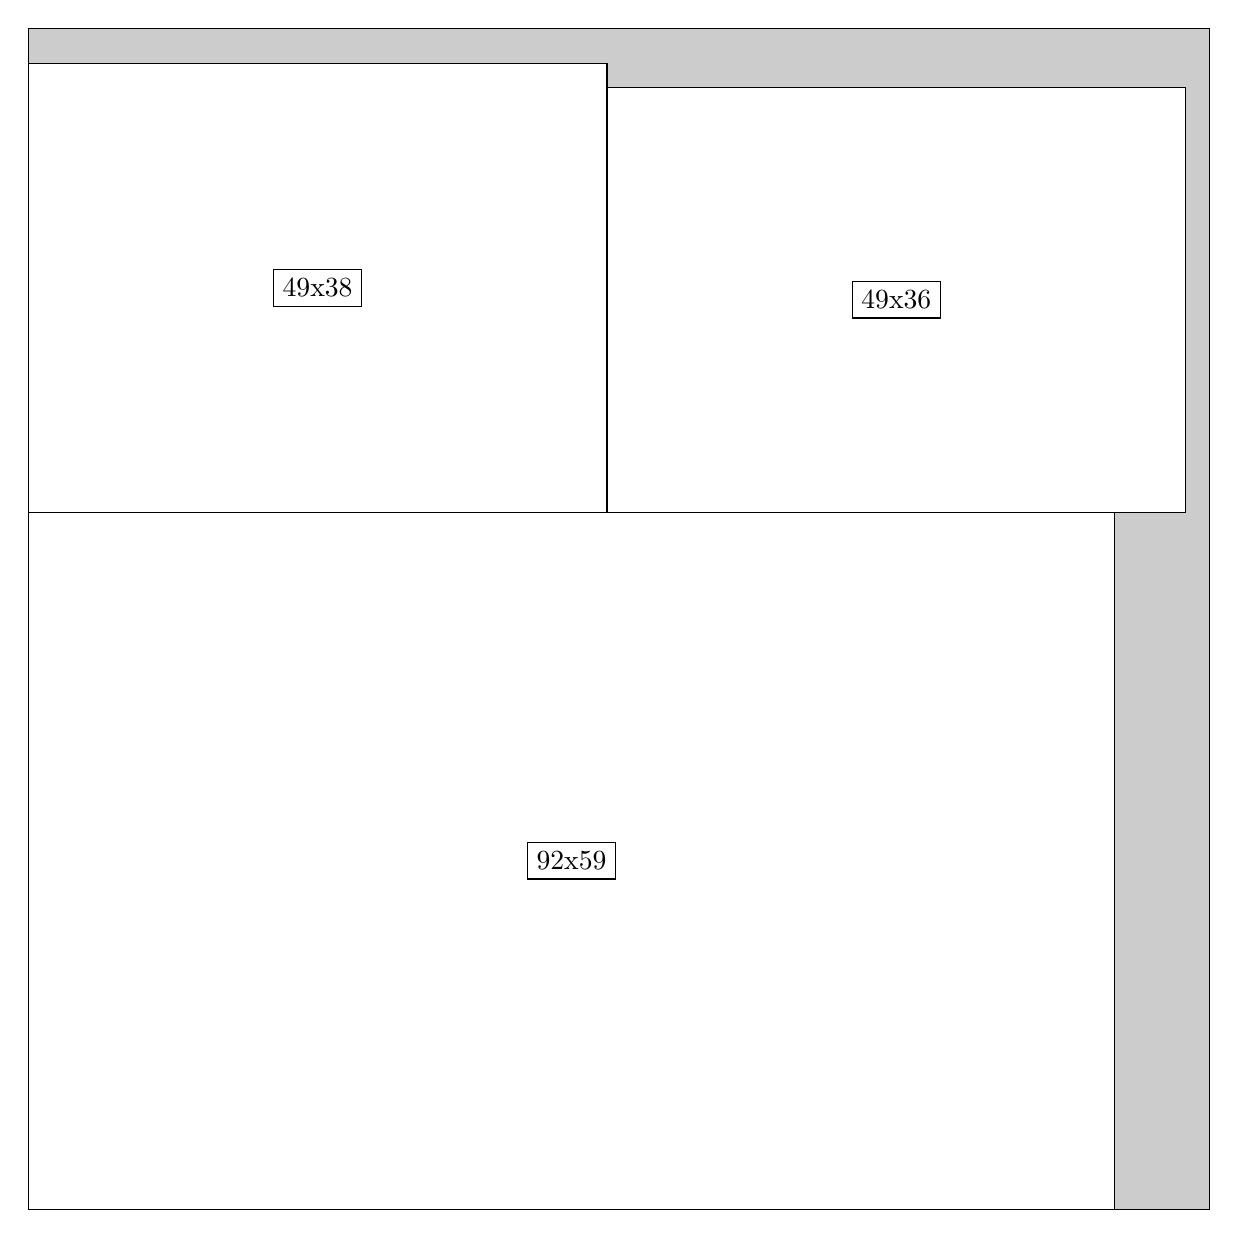
\begin{tikzpicture}[shorten >=1pt,scale=1.0,every node/.style={scale=1.0},->]
\tikzstyle{vertex}=[circle,fill=black!25,minimum size=14pt,inner sep=0pt]
\filldraw[fill=gray!40!white, draw=black] (0,0) rectangle (15.0,15.0);
\foreach \name/\x/\y/\w/\h in {92x59/0.0/0.0/13.799999999999999/8.85,49x38/0.0/8.85/7.35/5.7,49x36/7.35/8.85/7.35/5.3999999999999995}
\filldraw[fill=white!40!white, draw=black] (\x,\y) rectangle node[draw] (\name) {\name} ++(\w,\h);
\end{tikzpicture}


w =92 , h =59 , x =0 , y =0 , v =5428
\par
w =49 , h =38 , x =0 , y =59 , v =1862
\par
w =49 , h =36 , x =49 , y =59 , v =1764
\par
\newpage


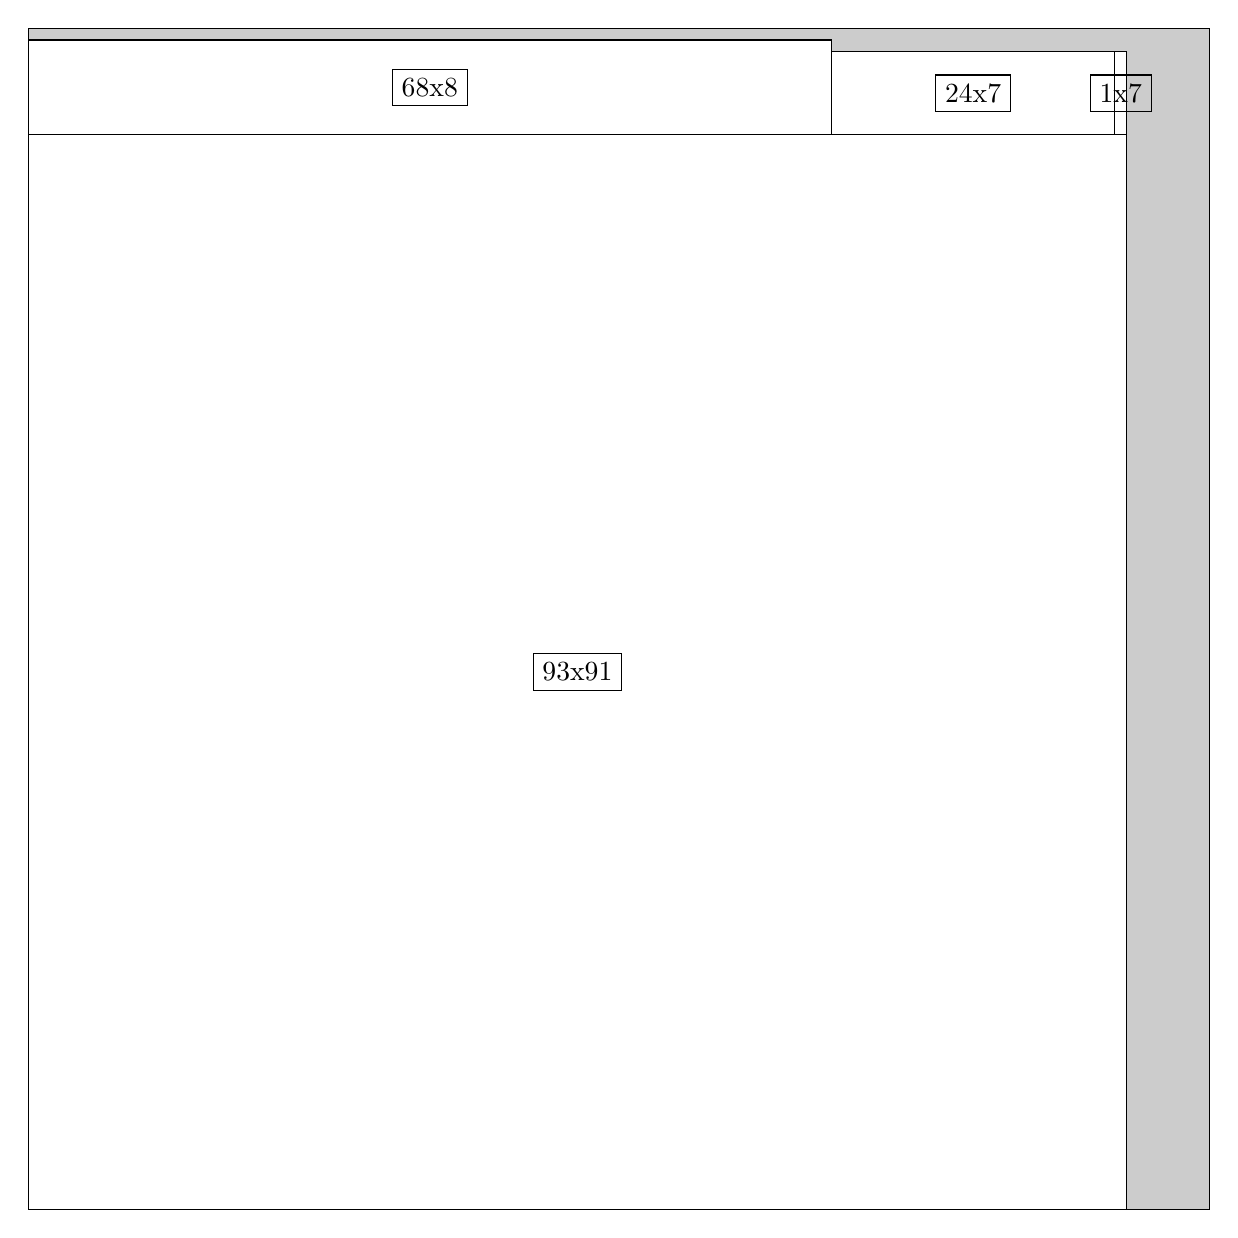
\begin{tikzpicture}[shorten >=1pt,scale=1.0,every node/.style={scale=1.0},->]
\tikzstyle{vertex}=[circle,fill=black!25,minimum size=14pt,inner sep=0pt]
\filldraw[fill=gray!40!white, draw=black] (0,0) rectangle (15.0,15.0);
\foreach \name/\x/\y/\w/\h in {93x91/0.0/0.0/13.95/13.65,24x7/10.2/13.65/3.5999999999999996/1.05,68x8/0.0/13.65/10.2/1.2,1x7/13.799999999999999/13.65/0.15/1.05}
\filldraw[fill=white!40!white, draw=black] (\x,\y) rectangle node[draw] (\name) {\name} ++(\w,\h);
\end{tikzpicture}


w =93 , h =91 , x =0 , y =0 , v =8463
\par
w =24 , h =7 , x =68 , y =91 , v =168
\par
w =68 , h =8 , x =0 , y =91 , v =544
\par
w =1 , h =7 , x =92 , y =91 , v =7
\par
\newpage


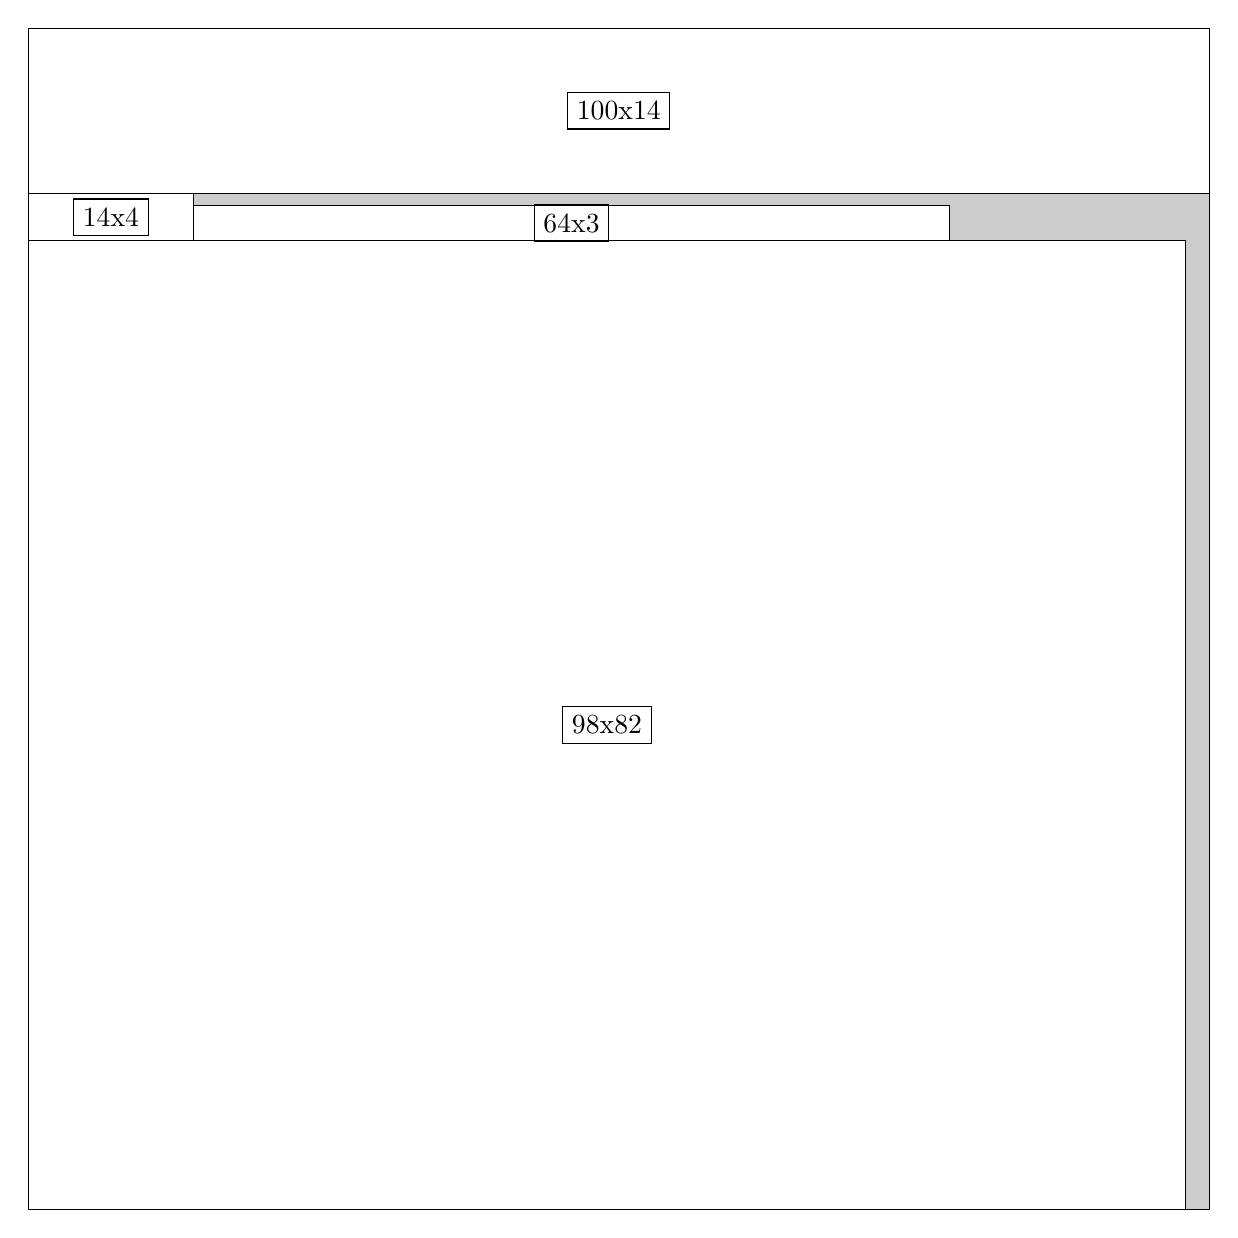
\begin{tikzpicture}[shorten >=1pt,scale=1.0,every node/.style={scale=1.0},->]
\tikzstyle{vertex}=[circle,fill=black!25,minimum size=14pt,inner sep=0pt]
\filldraw[fill=gray!40!white, draw=black] (0,0) rectangle (15.0,15.0);
\foreach \name/\x/\y/\w/\h in {98x82/0.0/0.0/14.7/12.299999999999999,100x14/0.0/12.9/15.0/2.1,64x3/2.1/12.299999999999999/9.6/0.44999999999999996,14x4/0.0/12.299999999999999/2.1/0.6}
\filldraw[fill=white!40!white, draw=black] (\x,\y) rectangle node[draw] (\name) {\name} ++(\w,\h);
\end{tikzpicture}


w =98 , h =82 , x =0 , y =0 , v =8036
\par
w =100 , h =14 , x =0 , y =86 , v =1400
\par
w =64 , h =3 , x =14 , y =82 , v =192
\par
w =14 , h =4 , x =0 , y =82 , v =56
\par
\newpage


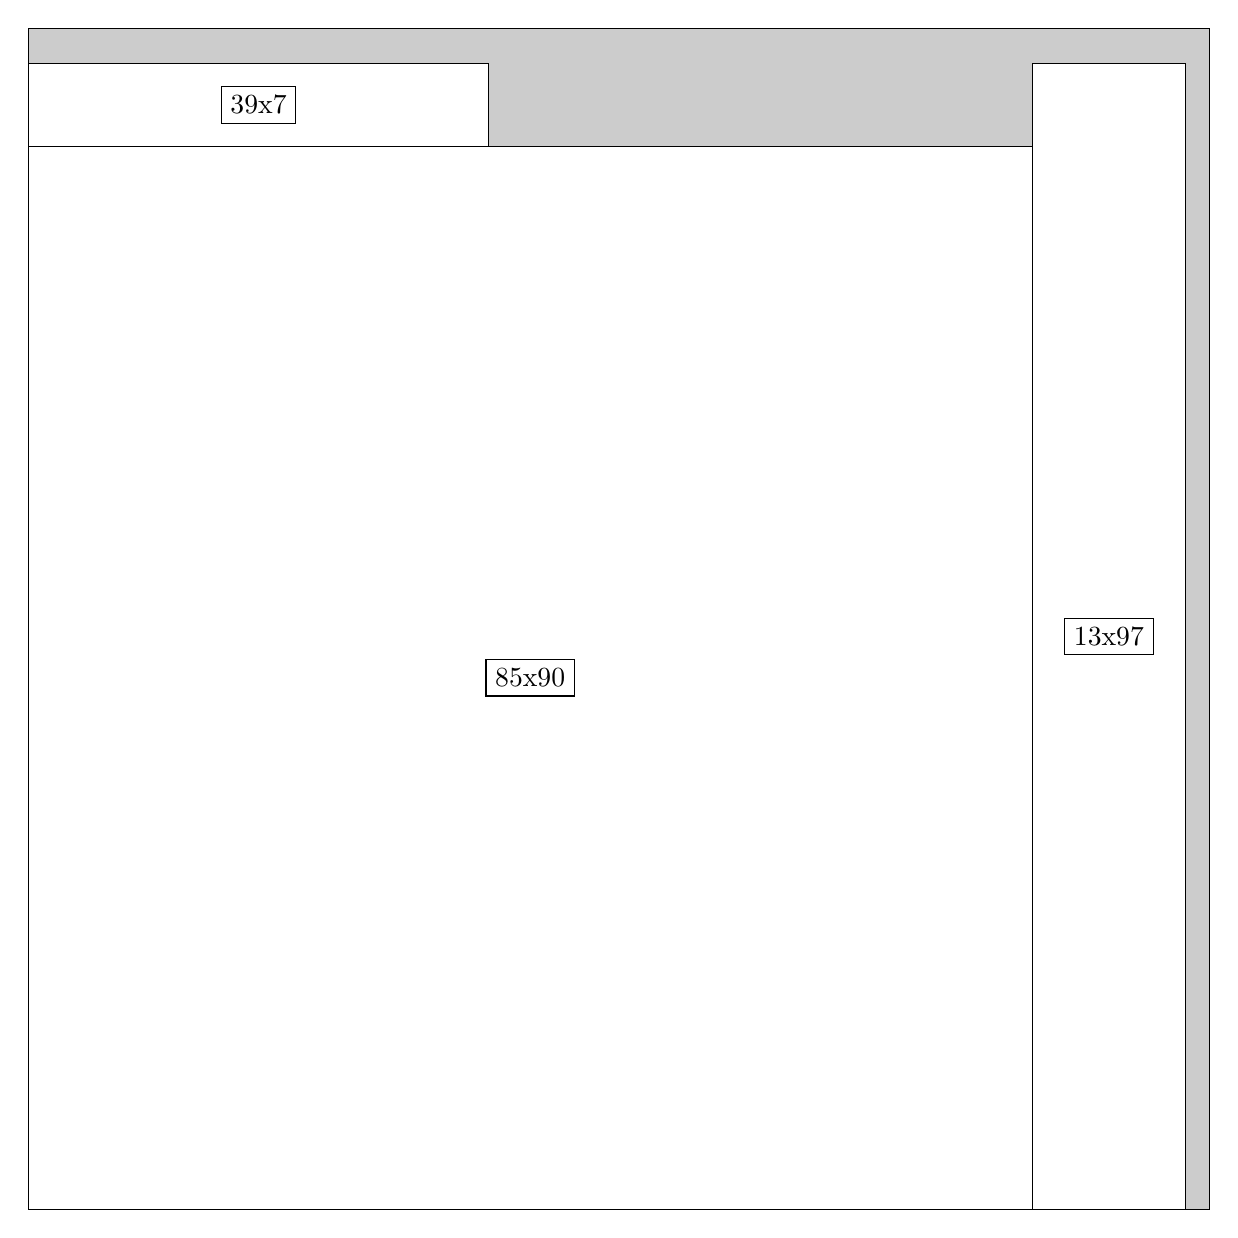
\begin{tikzpicture}[shorten >=1pt,scale=1.0,every node/.style={scale=1.0},->]
\tikzstyle{vertex}=[circle,fill=black!25,minimum size=14pt,inner sep=0pt]
\filldraw[fill=gray!40!white, draw=black] (0,0) rectangle (15.0,15.0);
\foreach \name/\x/\y/\w/\h in {85x90/0.0/0.0/12.75/13.5,13x97/12.75/0.0/1.95/14.549999999999999,39x7/0.0/13.5/5.85/1.05}
\filldraw[fill=white!40!white, draw=black] (\x,\y) rectangle node[draw] (\name) {\name} ++(\w,\h);
\end{tikzpicture}


w =85 , h =90 , x =0 , y =0 , v =7650
\par
w =13 , h =97 , x =85 , y =0 , v =1261
\par
w =39 , h =7 , x =0 , y =90 , v =273
\par
\newpage


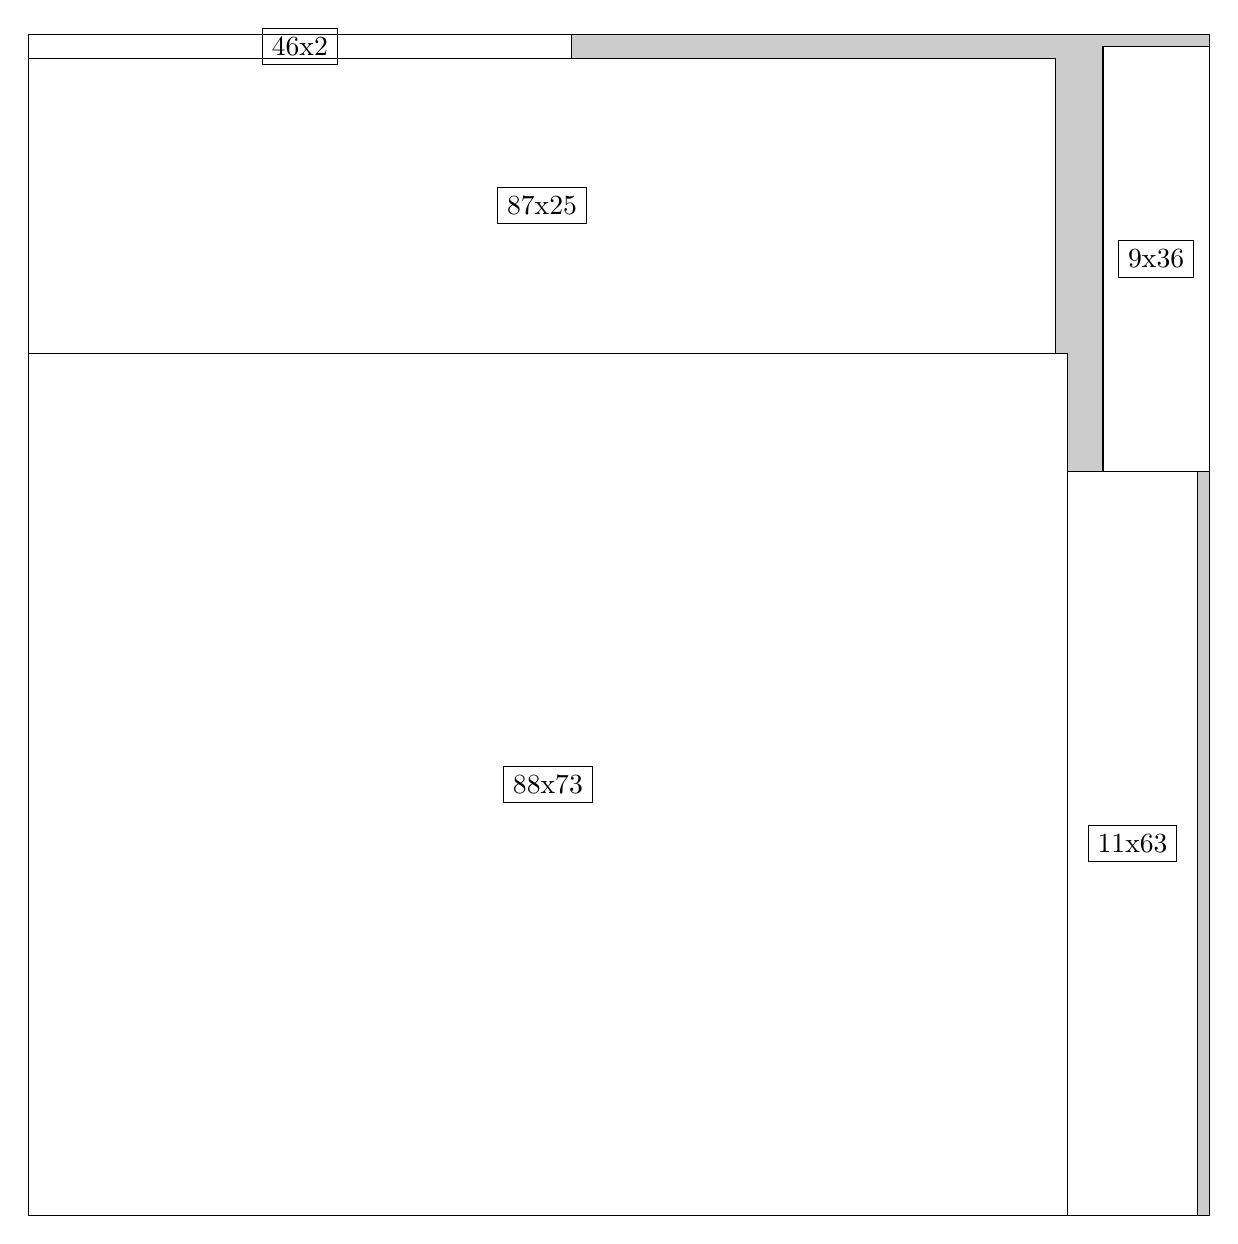
\begin{tikzpicture}[shorten >=1pt,scale=1.0,every node/.style={scale=1.0},->]
\tikzstyle{vertex}=[circle,fill=black!25,minimum size=14pt,inner sep=0pt]
\filldraw[fill=gray!40!white, draw=black] (0,0) rectangle (15.0,15.0);
\foreach \name/\x/\y/\w/\h in {88x73/0.0/0.0/13.2/10.95,87x25/0.0/10.95/13.049999999999999/3.75,11x63/13.2/0.0/1.65/9.45,9x36/13.65/9.45/1.3499999999999999/5.3999999999999995,46x2/0.0/14.7/6.8999999999999995/0.3}
\filldraw[fill=white!40!white, draw=black] (\x,\y) rectangle node[draw] (\name) {\name} ++(\w,\h);
\end{tikzpicture}


w =88 , h =73 , x =0 , y =0 , v =6424
\par
w =87 , h =25 , x =0 , y =73 , v =2175
\par
w =11 , h =63 , x =88 , y =0 , v =693
\par
w =9 , h =36 , x =91 , y =63 , v =324
\par
w =46 , h =2 , x =0 , y =98 , v =92
\par
\newpage


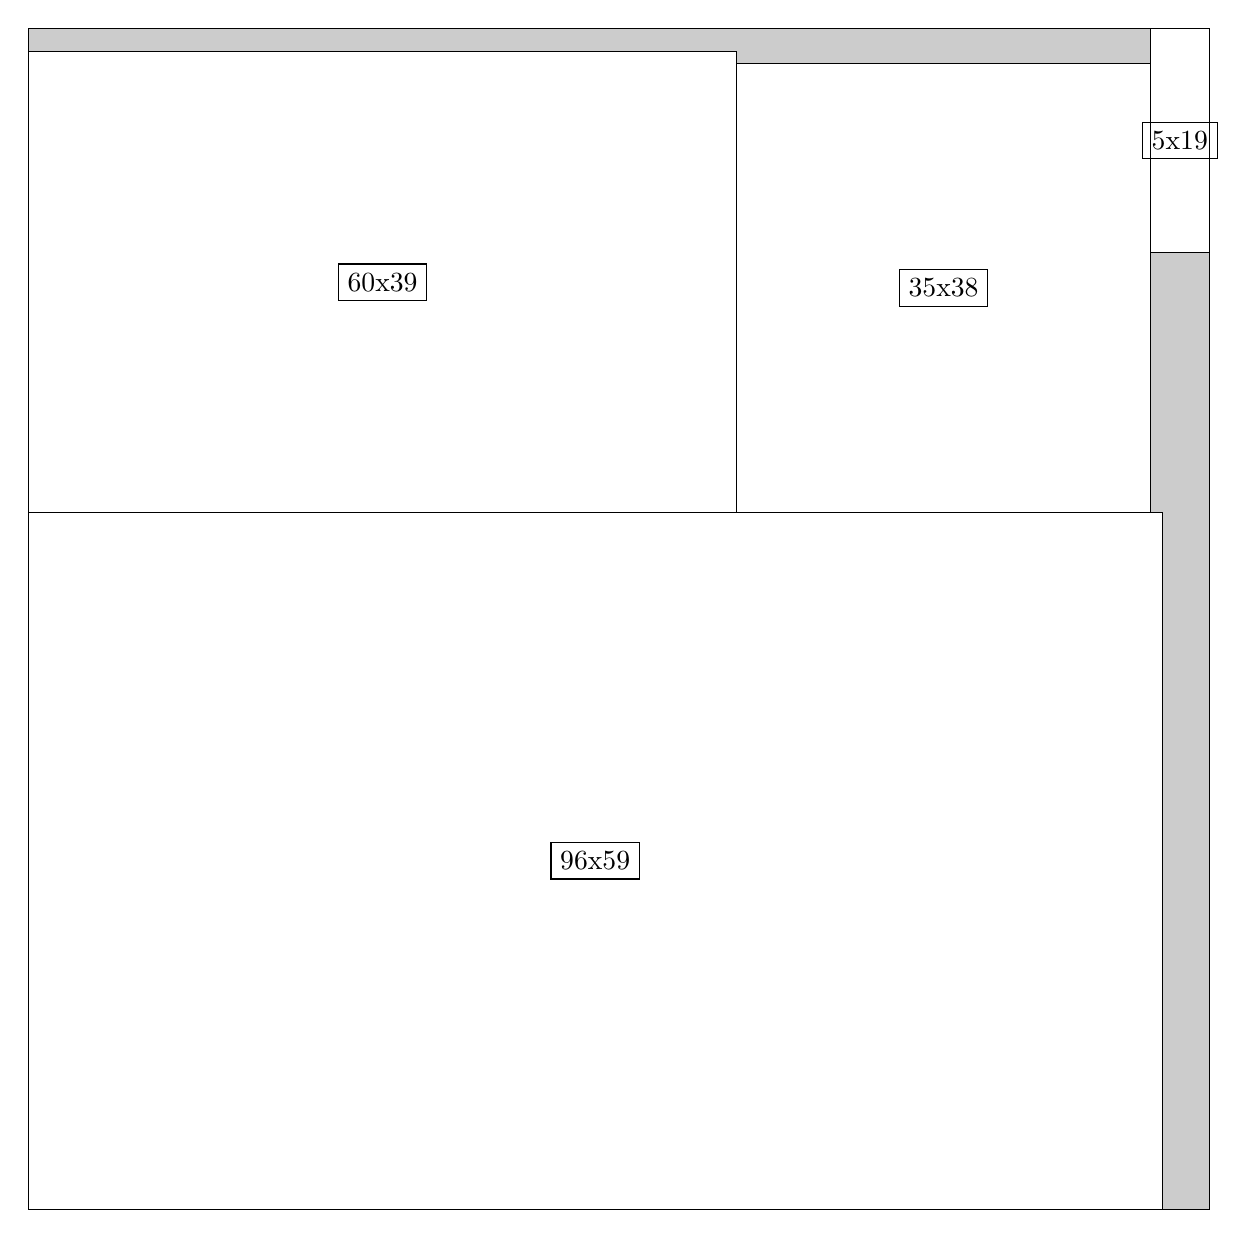
\begin{tikzpicture}[shorten >=1pt,scale=1.0,every node/.style={scale=1.0},->]
\tikzstyle{vertex}=[circle,fill=black!25,minimum size=14pt,inner sep=0pt]
\filldraw[fill=gray!40!white, draw=black] (0,0) rectangle (15.0,15.0);
\foreach \name/\x/\y/\w/\h in {96x59/0.0/0.0/14.399999999999999/8.85,60x39/0.0/8.85/9.0/5.85,35x38/9.0/8.85/5.25/5.7,5x19/14.25/12.15/0.75/2.85}
\filldraw[fill=white!40!white, draw=black] (\x,\y) rectangle node[draw] (\name) {\name} ++(\w,\h);
\end{tikzpicture}


w =96 , h =59 , x =0 , y =0 , v =5664
\par
w =60 , h =39 , x =0 , y =59 , v =2340
\par
w =35 , h =38 , x =60 , y =59 , v =1330
\par
w =5 , h =19 , x =95 , y =81 , v =95
\par
\newpage


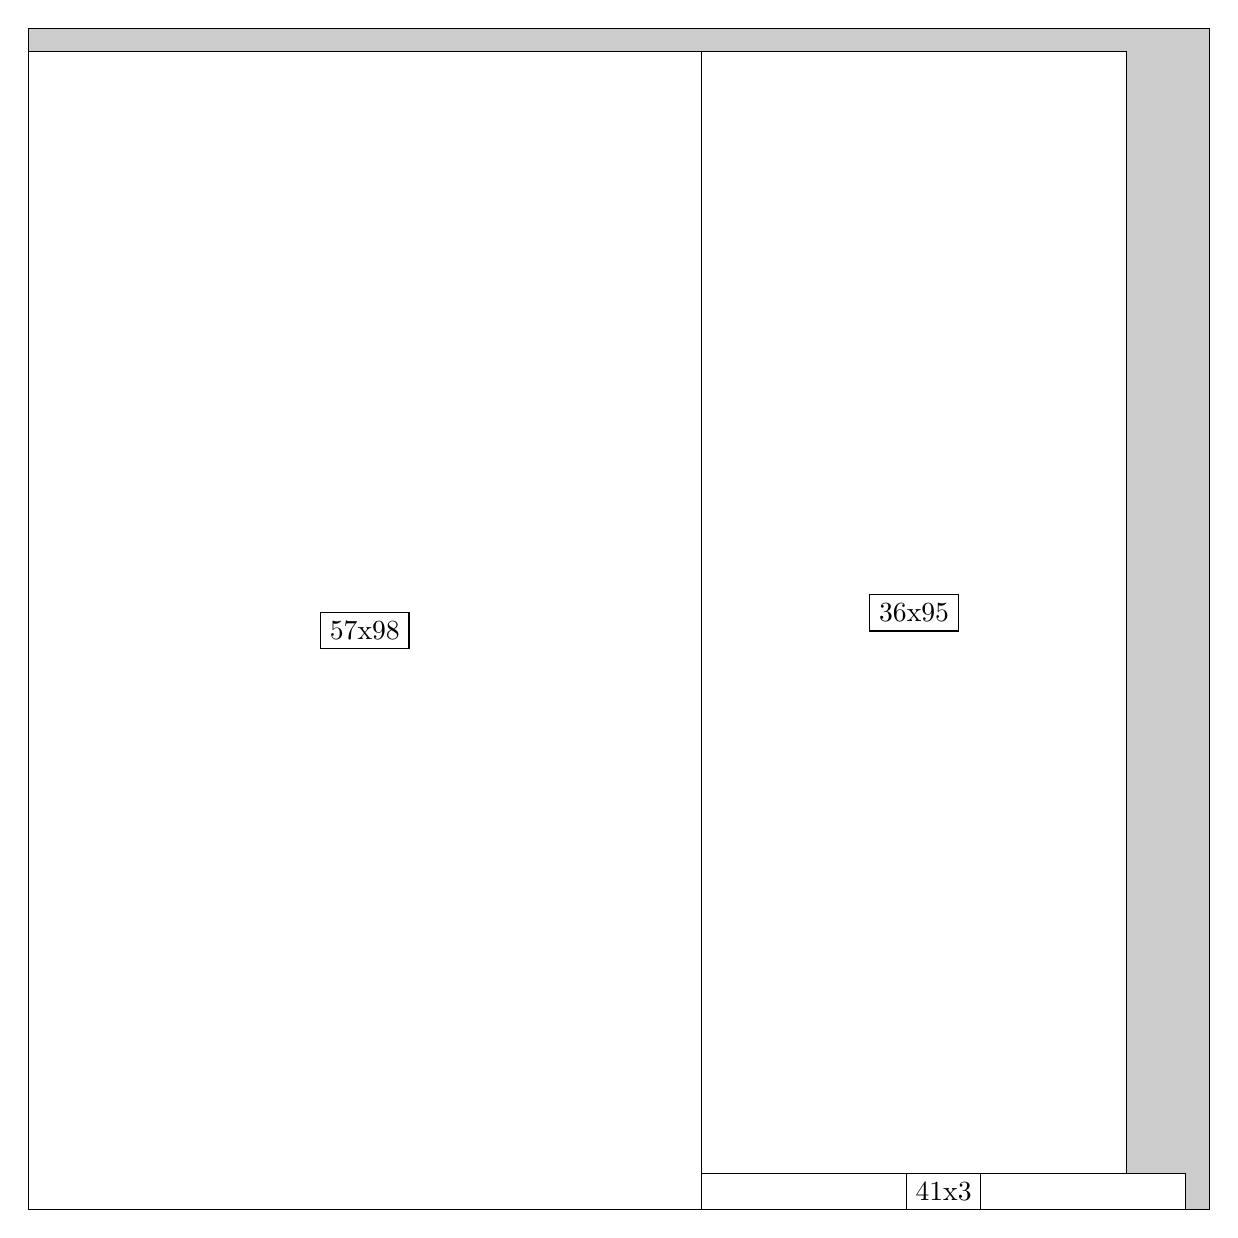
\begin{tikzpicture}[shorten >=1pt,scale=1.0,every node/.style={scale=1.0},->]
\tikzstyle{vertex}=[circle,fill=black!25,minimum size=14pt,inner sep=0pt]
\filldraw[fill=gray!40!white, draw=black] (0,0) rectangle (15.0,15.0);
\foreach \name/\x/\y/\w/\h in {57x98/0.0/0.0/8.549999999999999/14.7,36x95/8.549999999999999/0.44999999999999996/5.3999999999999995/14.25,41x3/8.549999999999999/0.0/6.1499999999999995/0.44999999999999996}
\filldraw[fill=white!40!white, draw=black] (\x,\y) rectangle node[draw] (\name) {\name} ++(\w,\h);
\end{tikzpicture}


w =57 , h =98 , x =0 , y =0 , v =5586
\par
w =36 , h =95 , x =57 , y =3 , v =3420
\par
w =41 , h =3 , x =57 , y =0 , v =123
\par
\newpage


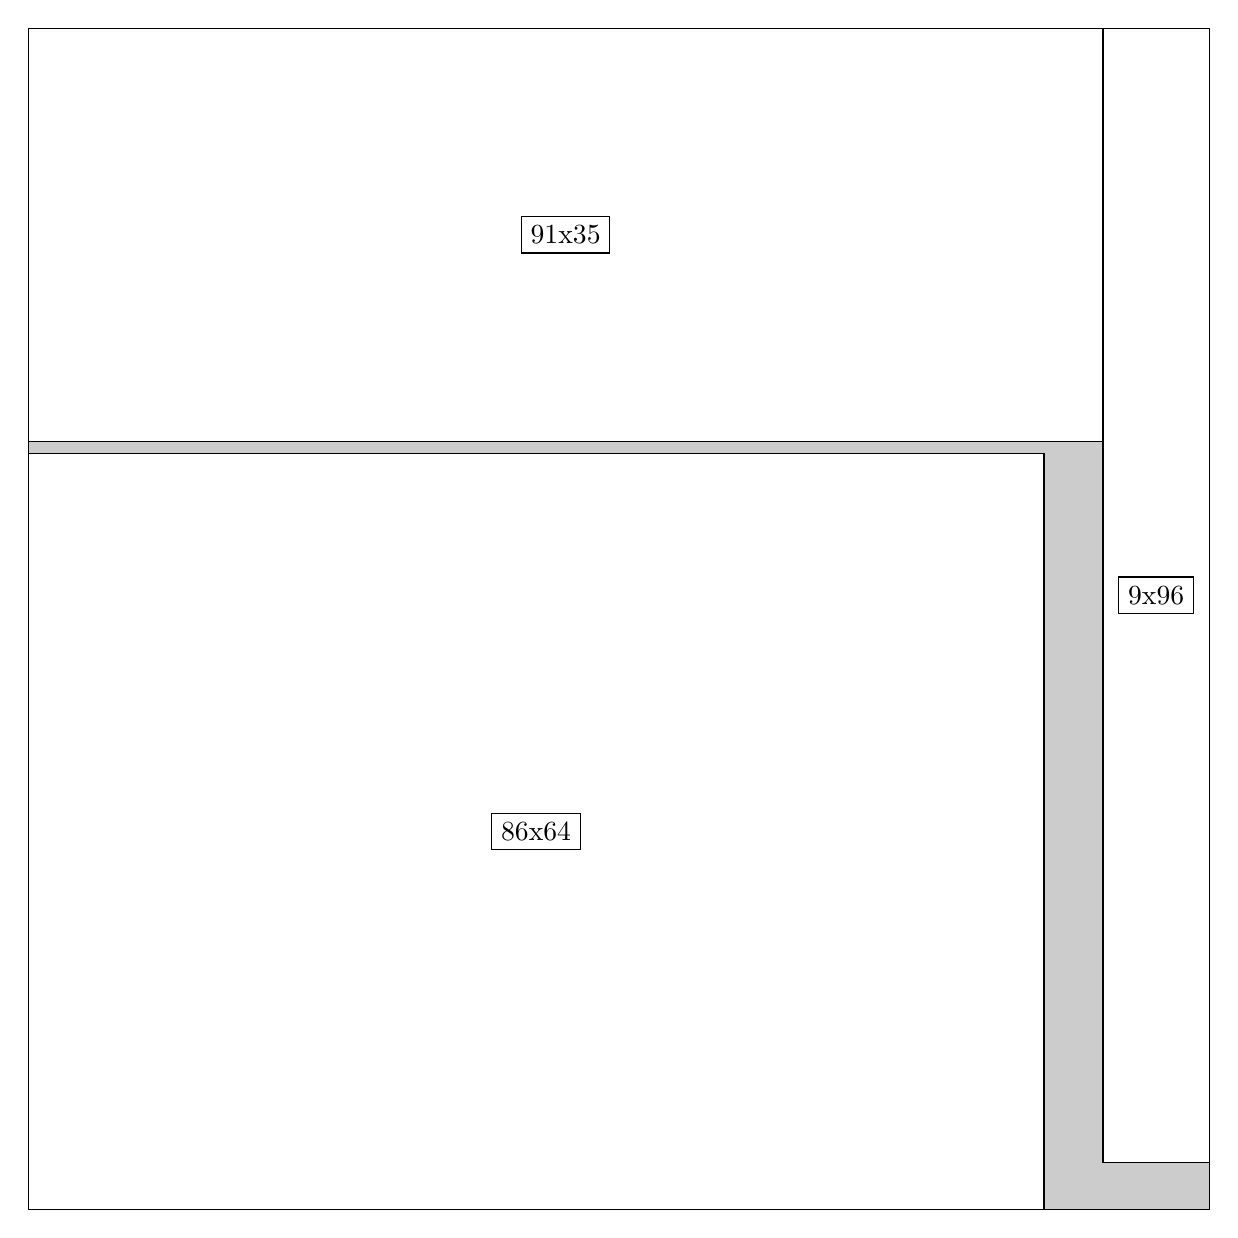
\begin{tikzpicture}[shorten >=1pt,scale=1.0,every node/.style={scale=1.0},->]
\tikzstyle{vertex}=[circle,fill=black!25,minimum size=14pt,inner sep=0pt]
\filldraw[fill=gray!40!white, draw=black] (0,0) rectangle (15.0,15.0);
\foreach \name/\x/\y/\w/\h in {86x64/0.0/0.0/12.9/9.6,91x35/0.0/9.75/13.65/5.25,9x96/13.65/0.6/1.3499999999999999/14.399999999999999}
\filldraw[fill=white!40!white, draw=black] (\x,\y) rectangle node[draw] (\name) {\name} ++(\w,\h);
\end{tikzpicture}


w =86 , h =64 , x =0 , y =0 , v =5504
\par
w =91 , h =35 , x =0 , y =65 , v =3185
\par
w =9 , h =96 , x =91 , y =4 , v =864
\par
\newpage


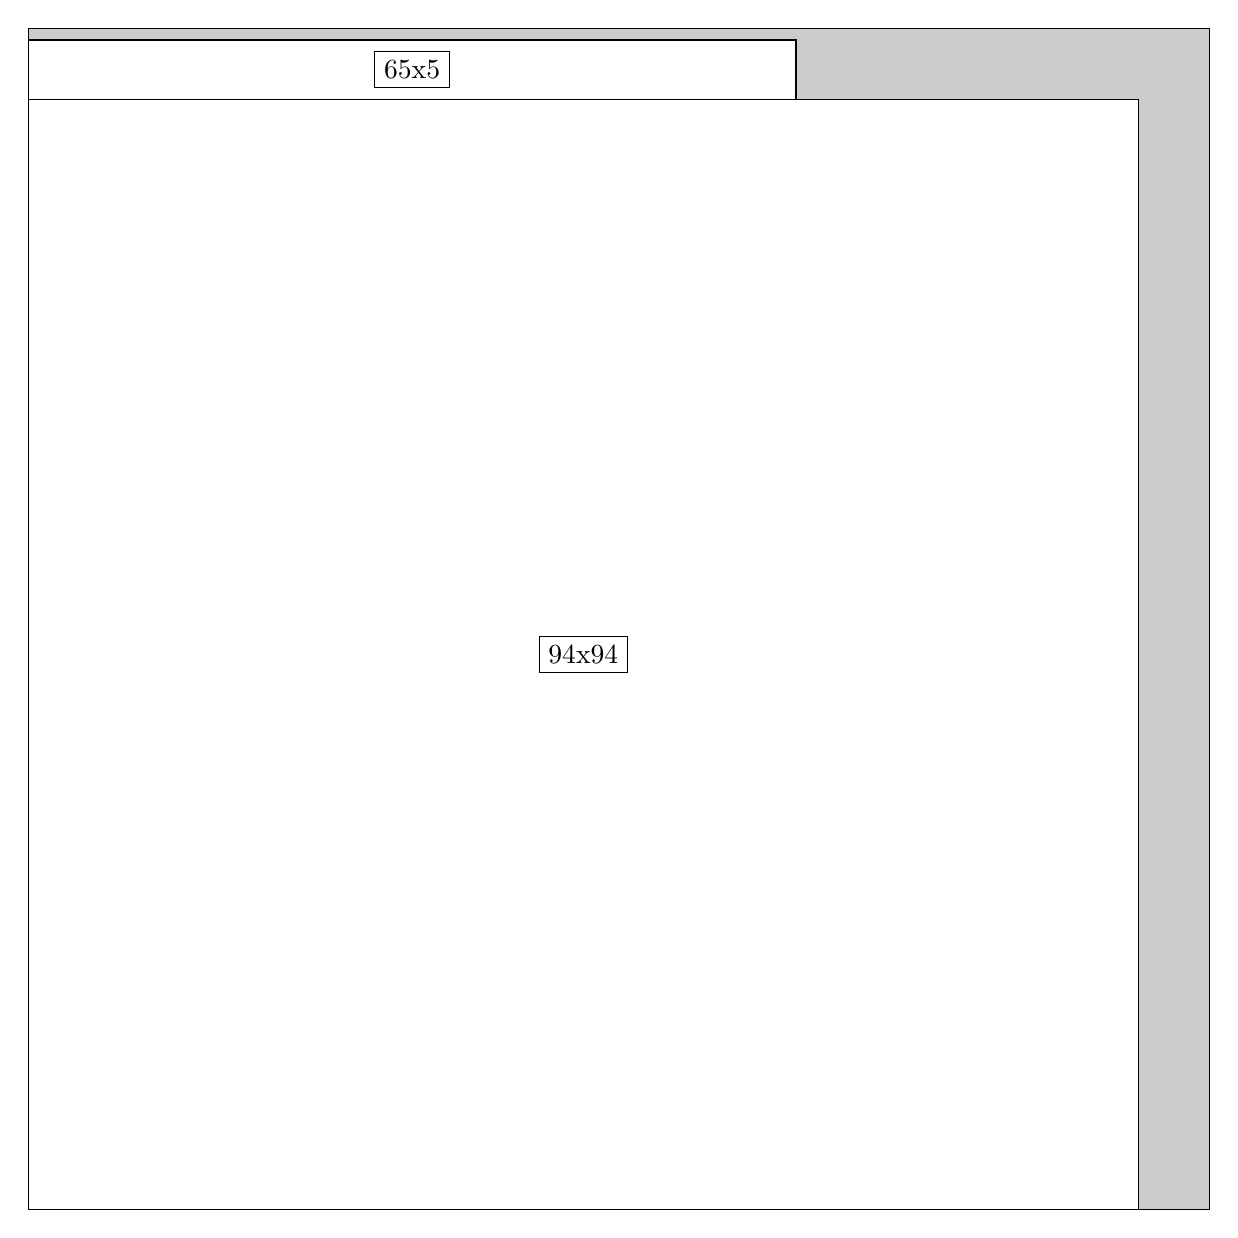
\begin{tikzpicture}[shorten >=1pt,scale=1.0,every node/.style={scale=1.0},->]
\tikzstyle{vertex}=[circle,fill=black!25,minimum size=14pt,inner sep=0pt]
\filldraw[fill=gray!40!white, draw=black] (0,0) rectangle (15.0,15.0);
\foreach \name/\x/\y/\w/\h in {94x94/0.0/0.0/14.1/14.1,65x5/0.0/14.1/9.75/0.75}
\filldraw[fill=white!40!white, draw=black] (\x,\y) rectangle node[draw] (\name) {\name} ++(\w,\h);
\end{tikzpicture}


w =94 , h =94 , x =0 , y =0 , v =8836
\par
w =65 , h =5 , x =0 , y =94 , v =325
\par
\newpage


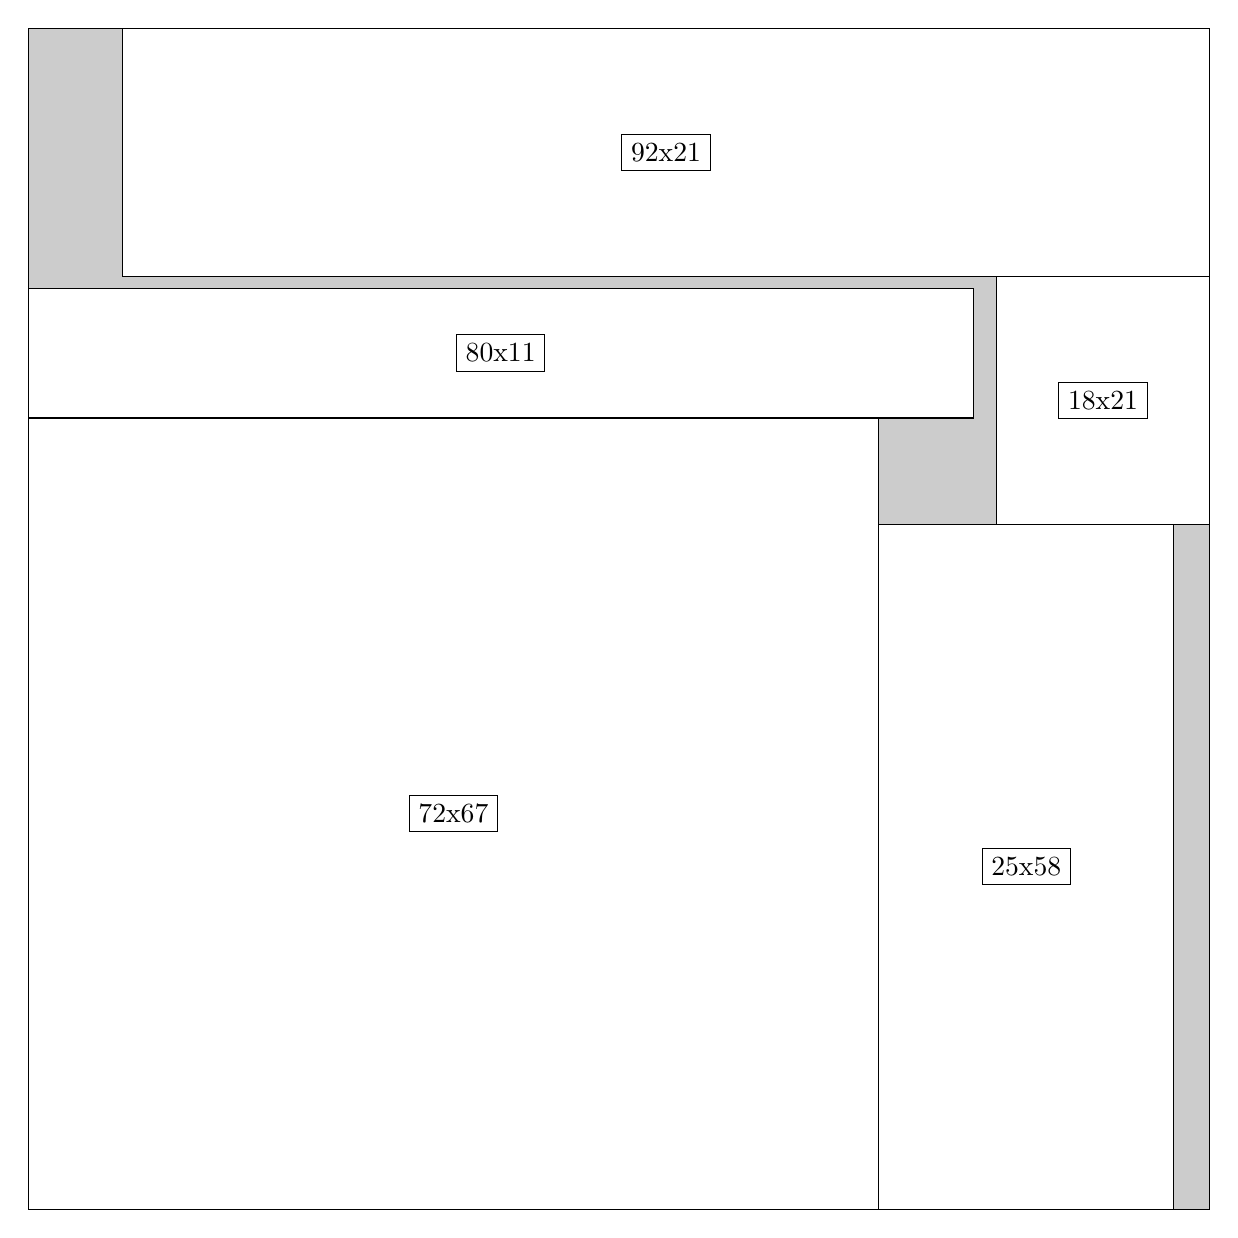
\begin{tikzpicture}[shorten >=1pt,scale=1.0,every node/.style={scale=1.0},->]
\tikzstyle{vertex}=[circle,fill=black!25,minimum size=14pt,inner sep=0pt]
\filldraw[fill=gray!40!white, draw=black] (0,0) rectangle (15.0,15.0);
\foreach \name/\x/\y/\w/\h in {72x67/0.0/0.0/10.799999999999999/10.049999999999999,92x21/1.2/11.85/13.799999999999999/3.15,25x58/10.799999999999999/0.0/3.75/8.7,80x11/0.0/10.049999999999999/12.0/1.65,18x21/12.299999999999999/8.7/2.6999999999999997/3.15}
\filldraw[fill=white!40!white, draw=black] (\x,\y) rectangle node[draw] (\name) {\name} ++(\w,\h);
\end{tikzpicture}


w =72 , h =67 , x =0 , y =0 , v =4824
\par
w =92 , h =21 , x =8 , y =79 , v =1932
\par
w =25 , h =58 , x =72 , y =0 , v =1450
\par
w =80 , h =11 , x =0 , y =67 , v =880
\par
w =18 , h =21 , x =82 , y =58 , v =378
\par
\newpage


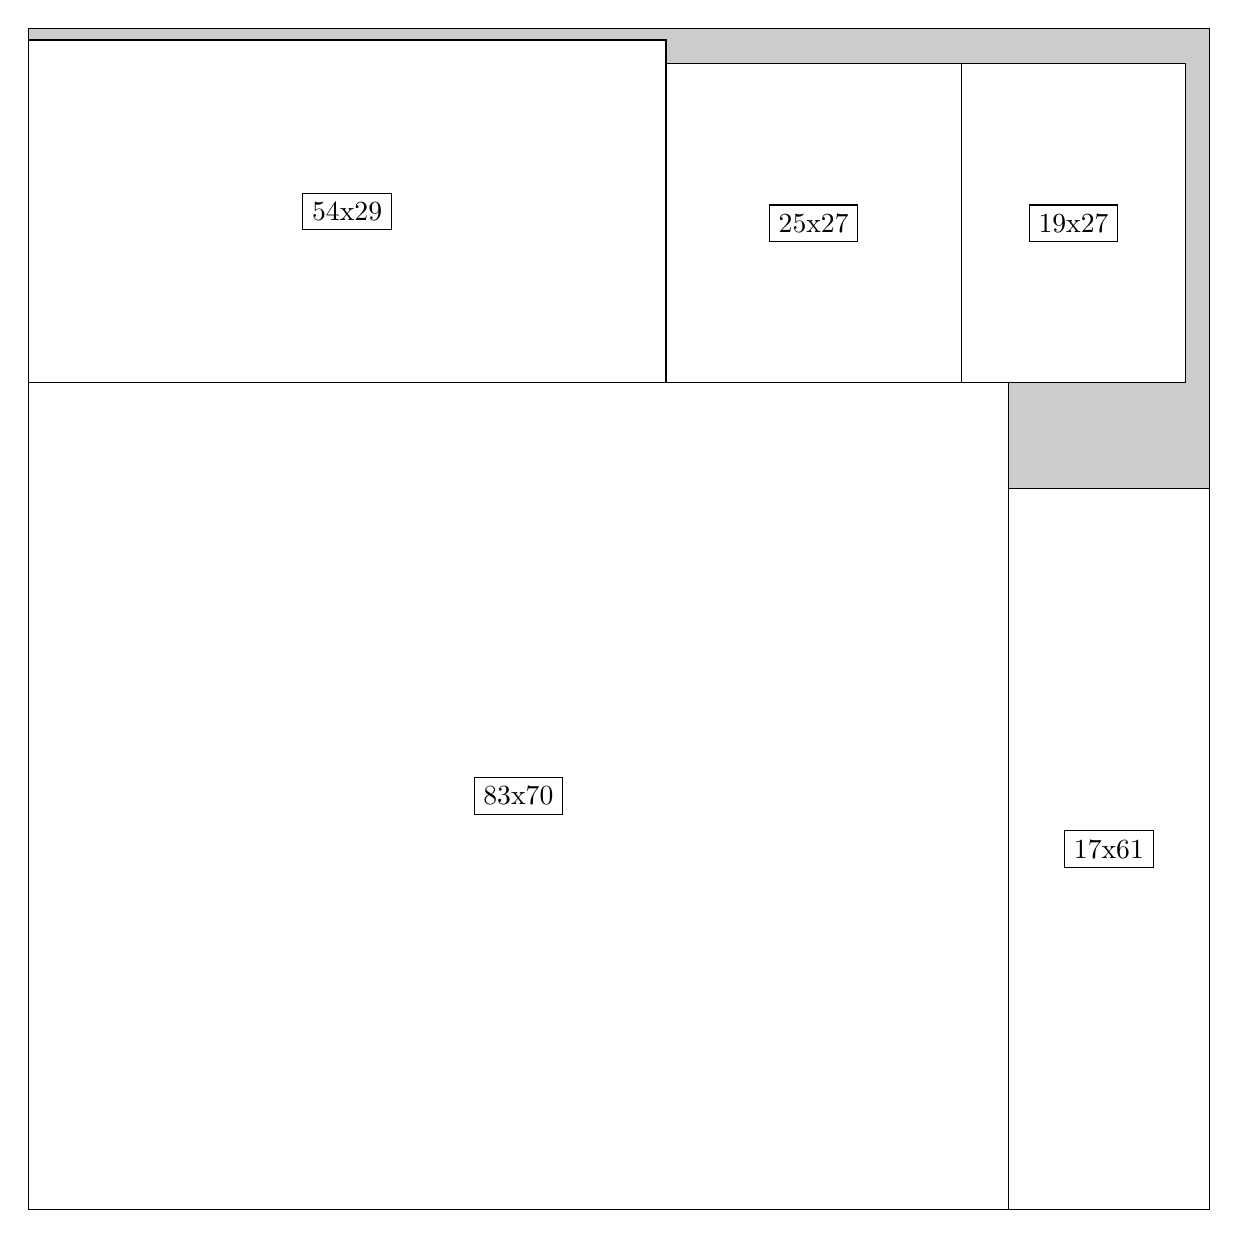
\begin{tikzpicture}[shorten >=1pt,scale=1.0,every node/.style={scale=1.0},->]
\tikzstyle{vertex}=[circle,fill=black!25,minimum size=14pt,inner sep=0pt]
\filldraw[fill=gray!40!white, draw=black] (0,0) rectangle (15.0,15.0);
\foreach \name/\x/\y/\w/\h in {83x70/0.0/0.0/12.45/10.5,54x29/0.0/10.5/8.1/4.35,17x61/12.45/0.0/2.55/9.15,25x27/8.1/10.5/3.75/4.05,19x27/11.85/10.5/2.85/4.05}
\filldraw[fill=white!40!white, draw=black] (\x,\y) rectangle node[draw] (\name) {\name} ++(\w,\h);
\end{tikzpicture}


w =83 , h =70 , x =0 , y =0 , v =5810
\par
w =54 , h =29 , x =0 , y =70 , v =1566
\par
w =17 , h =61 , x =83 , y =0 , v =1037
\par
w =25 , h =27 , x =54 , y =70 , v =675
\par
w =19 , h =27 , x =79 , y =70 , v =513
\par
\newpage


\begin{tikzpicture}[shorten >=1pt,scale=1.0,every node/.style={scale=1.0},->]
\tikzstyle{vertex}=[circle,fill=black!25,minimum size=14pt,inner sep=0pt]
\filldraw[fill=gray!40!white, draw=black] (0,0) rectangle (15.0,15.0);
\foreach \name/\x/\y/\w/\h in {68x75/0.0/0.0/10.2/11.25,98x24/0.0/11.4/14.7/3.5999999999999996,32x75/10.2/0.0/4.8/11.25}
\filldraw[fill=white!40!white, draw=black] (\x,\y) rectangle node[draw] (\name) {\name} ++(\w,\h);
\end{tikzpicture}


w =68 , h =75 , x =0 , y =0 , v =5100
\par
w =98 , h =24 , x =0 , y =76 , v =2352
\par
w =32 , h =75 , x =68 , y =0 , v =2400
\par
\newpage


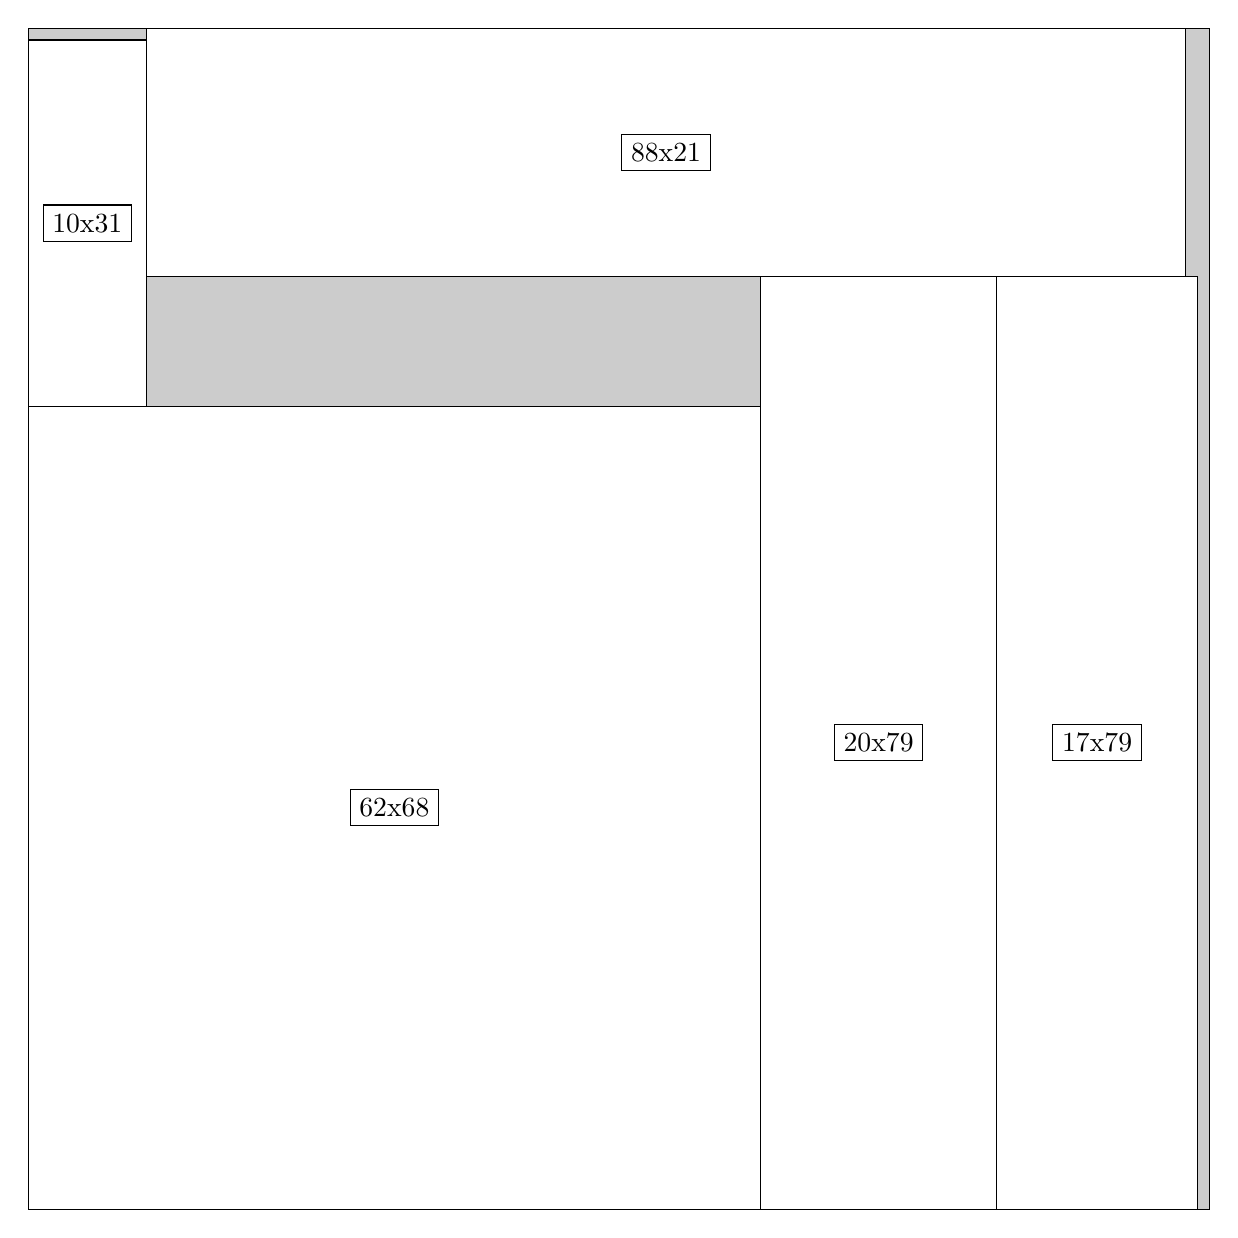
\begin{tikzpicture}[shorten >=1pt,scale=1.0,every node/.style={scale=1.0},->]
\tikzstyle{vertex}=[circle,fill=black!25,minimum size=14pt,inner sep=0pt]
\filldraw[fill=gray!40!white, draw=black] (0,0) rectangle (15.0,15.0);
\foreach \name/\x/\y/\w/\h in {62x68/0.0/0.0/9.299999999999999/10.2,88x21/1.5/11.85/13.2/3.15,20x79/9.299999999999999/0.0/3.0/11.85,17x79/12.299999999999999/0.0/2.55/11.85,10x31/0.0/10.2/1.5/4.6499999999999995}
\filldraw[fill=white!40!white, draw=black] (\x,\y) rectangle node[draw] (\name) {\name} ++(\w,\h);
\end{tikzpicture}


w =62 , h =68 , x =0 , y =0 , v =4216
\par
w =88 , h =21 , x =10 , y =79 , v =1848
\par
w =20 , h =79 , x =62 , y =0 , v =1580
\par
w =17 , h =79 , x =82 , y =0 , v =1343
\par
w =10 , h =31 , x =0 , y =68 , v =310
\par
\newpage


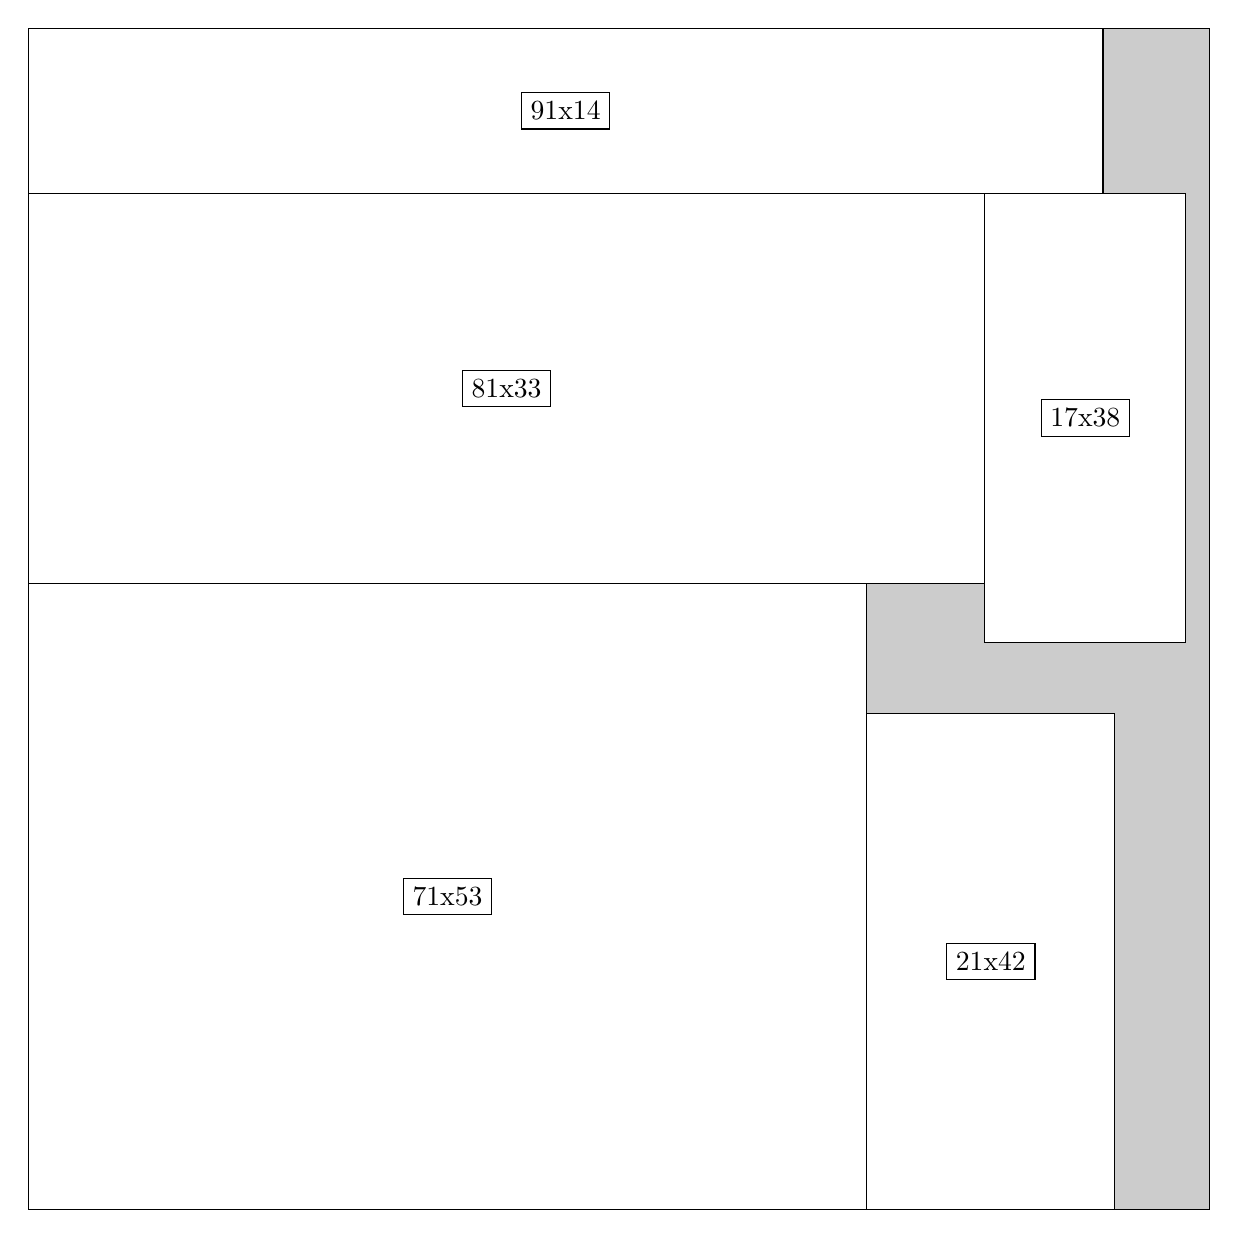
\begin{tikzpicture}[shorten >=1pt,scale=1.0,every node/.style={scale=1.0},->]
\tikzstyle{vertex}=[circle,fill=black!25,minimum size=14pt,inner sep=0pt]
\filldraw[fill=gray!40!white, draw=black] (0,0) rectangle (15.0,15.0);
\foreach \name/\x/\y/\w/\h in {81x33/0.0/7.949999999999999/12.15/4.95,71x53/0.0/0.0/10.65/7.949999999999999,91x14/0.0/12.9/13.65/2.1,21x42/10.65/0.0/3.15/6.3,17x38/12.15/7.199999999999999/2.55/5.7}
\filldraw[fill=white!40!white, draw=black] (\x,\y) rectangle node[draw] (\name) {\name} ++(\w,\h);
\end{tikzpicture}


w =81 , h =33 , x =0 , y =53 , v =2673
\par
w =71 , h =53 , x =0 , y =0 , v =3763
\par
w =91 , h =14 , x =0 , y =86 , v =1274
\par
w =21 , h =42 , x =71 , y =0 , v =882
\par
w =17 , h =38 , x =81 , y =48 , v =646
\par
\newpage


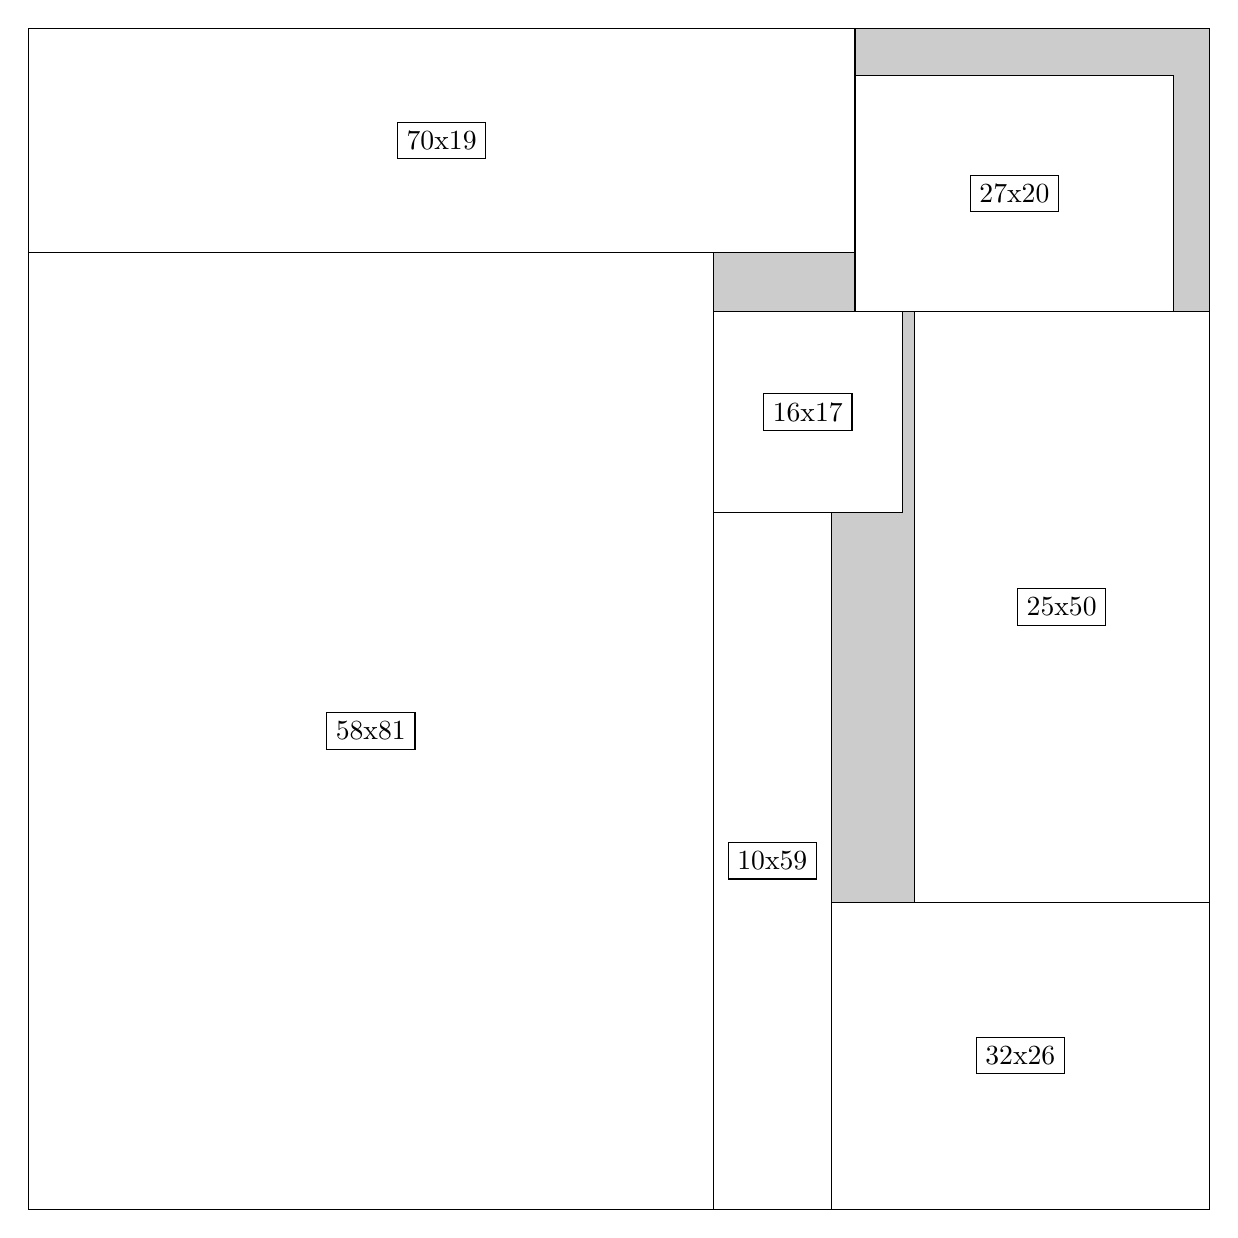
\begin{tikzpicture}[shorten >=1pt,scale=1.0,every node/.style={scale=1.0},->]
\tikzstyle{vertex}=[circle,fill=black!25,minimum size=14pt,inner sep=0pt]
\filldraw[fill=gray!40!white, draw=black] (0,0) rectangle (15.0,15.0);
\foreach \name/\x/\y/\w/\h in {32x26/10.2/0.0/4.8/3.9,58x81/0.0/0.0/8.7/12.15,70x19/0.0/12.15/10.5/2.85,25x50/11.25/3.9/3.75/7.5,10x59/8.7/0.0/1.5/8.85,27x20/10.5/11.4/4.05/3.0,16x17/8.7/8.85/2.4/2.55}
\filldraw[fill=white!40!white, draw=black] (\x,\y) rectangle node[draw] (\name) {\name} ++(\w,\h);
\end{tikzpicture}


w =32 , h =26 , x =68 , y =0 , v =832
\par
w =58 , h =81 , x =0 , y =0 , v =4698
\par
w =70 , h =19 , x =0 , y =81 , v =1330
\par
w =25 , h =50 , x =75 , y =26 , v =1250
\par
w =10 , h =59 , x =58 , y =0 , v =590
\par
w =27 , h =20 , x =70 , y =76 , v =540
\par
w =16 , h =17 , x =58 , y =59 , v =272
\par
\newpage


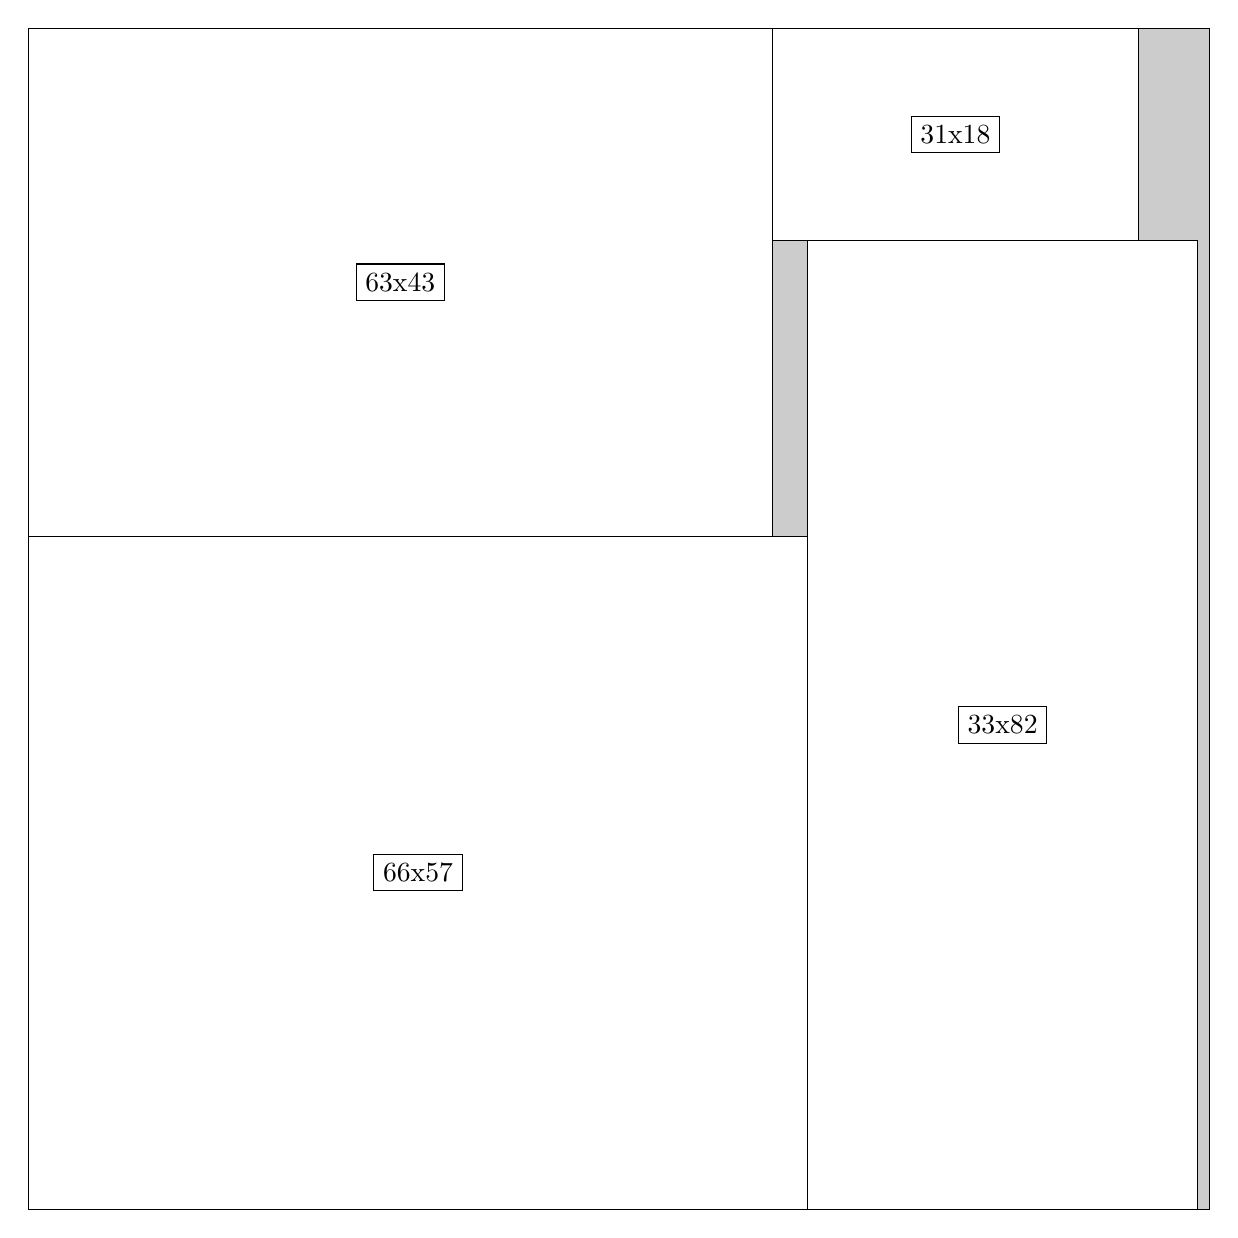
\begin{tikzpicture}[shorten >=1pt,scale=1.0,every node/.style={scale=1.0},->]
\tikzstyle{vertex}=[circle,fill=black!25,minimum size=14pt,inner sep=0pt]
\filldraw[fill=gray!40!white, draw=black] (0,0) rectangle (15.0,15.0);
\foreach \name/\x/\y/\w/\h in {66x57/0.0/0.0/9.9/8.549999999999999,63x43/0.0/8.549999999999999/9.45/6.45,33x82/9.9/0.0/4.95/12.299999999999999,31x18/9.45/12.299999999999999/4.6499999999999995/2.6999999999999997}
\filldraw[fill=white!40!white, draw=black] (\x,\y) rectangle node[draw] (\name) {\name} ++(\w,\h);
\end{tikzpicture}


w =66 , h =57 , x =0 , y =0 , v =3762
\par
w =63 , h =43 , x =0 , y =57 , v =2709
\par
w =33 , h =82 , x =66 , y =0 , v =2706
\par
w =31 , h =18 , x =63 , y =82 , v =558
\par
\newpage


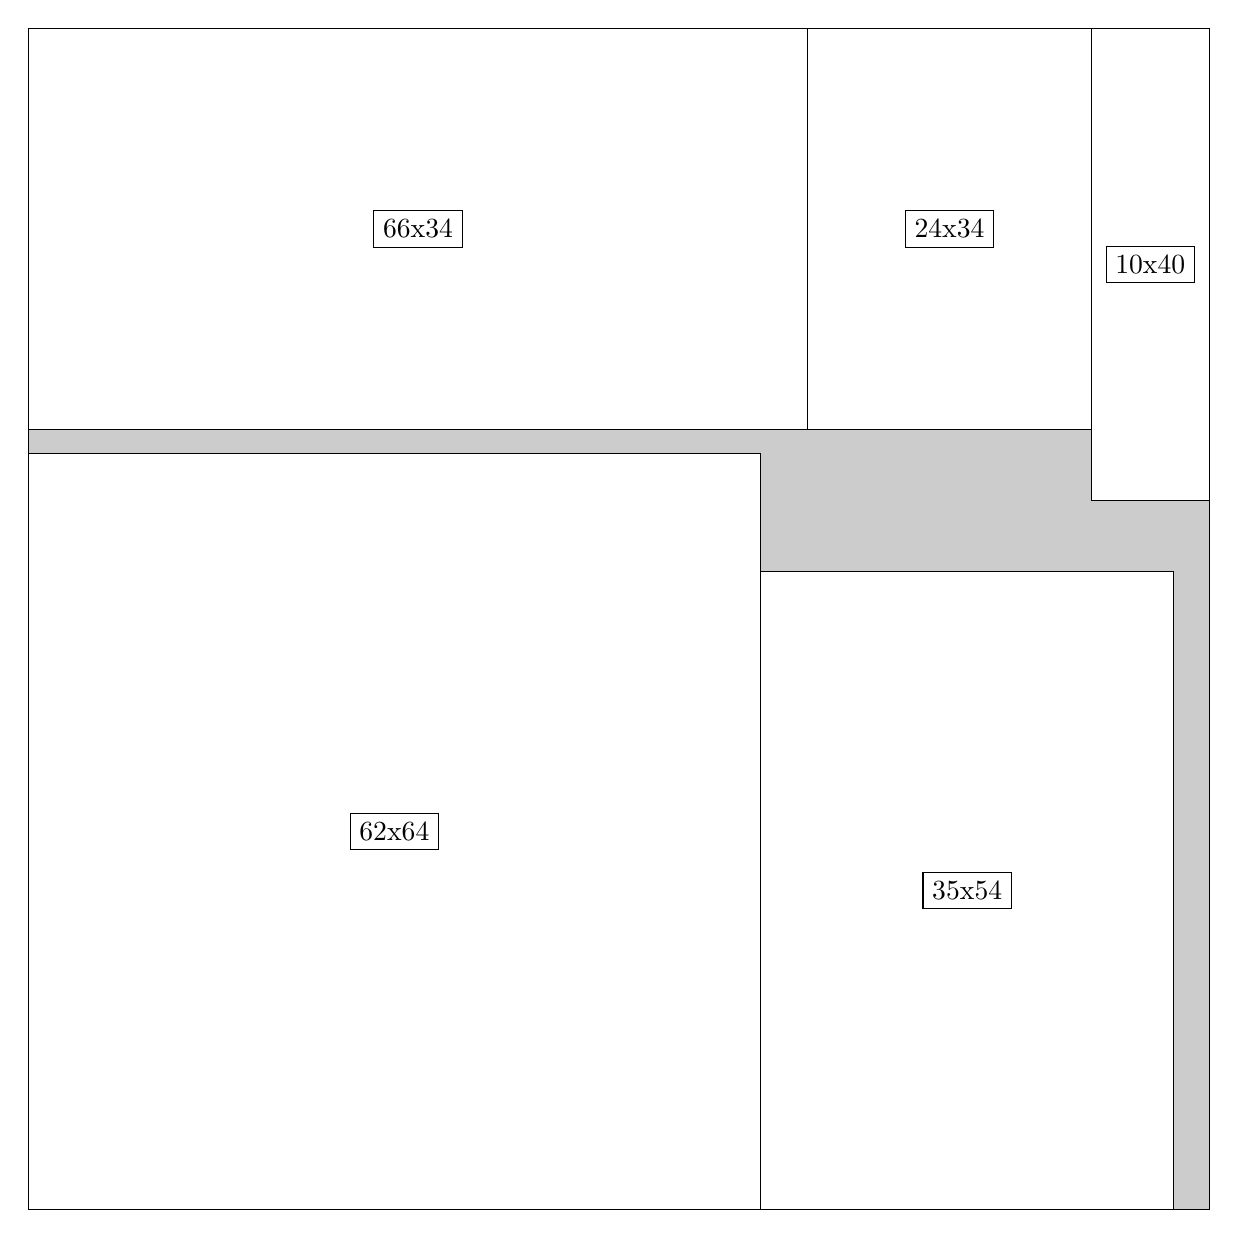
\begin{tikzpicture}[shorten >=1pt,scale=1.0,every node/.style={scale=1.0},->]
\tikzstyle{vertex}=[circle,fill=black!25,minimum size=14pt,inner sep=0pt]
\filldraw[fill=gray!40!white, draw=black] (0,0) rectangle (15.0,15.0);
\foreach \name/\x/\y/\w/\h in {62x64/0.0/0.0/9.299999999999999/9.6,66x34/0.0/9.9/9.9/5.1,35x54/9.299999999999999/0.0/5.25/8.1,24x34/9.9/9.9/3.5999999999999996/5.1,10x40/13.5/9.0/1.5/6.0}
\filldraw[fill=white!40!white, draw=black] (\x,\y) rectangle node[draw] (\name) {\name} ++(\w,\h);
\end{tikzpicture}


w =62 , h =64 , x =0 , y =0 , v =3968
\par
w =66 , h =34 , x =0 , y =66 , v =2244
\par
w =35 , h =54 , x =62 , y =0 , v =1890
\par
w =24 , h =34 , x =66 , y =66 , v =816
\par
w =10 , h =40 , x =90 , y =60 , v =400
\par
\newpage


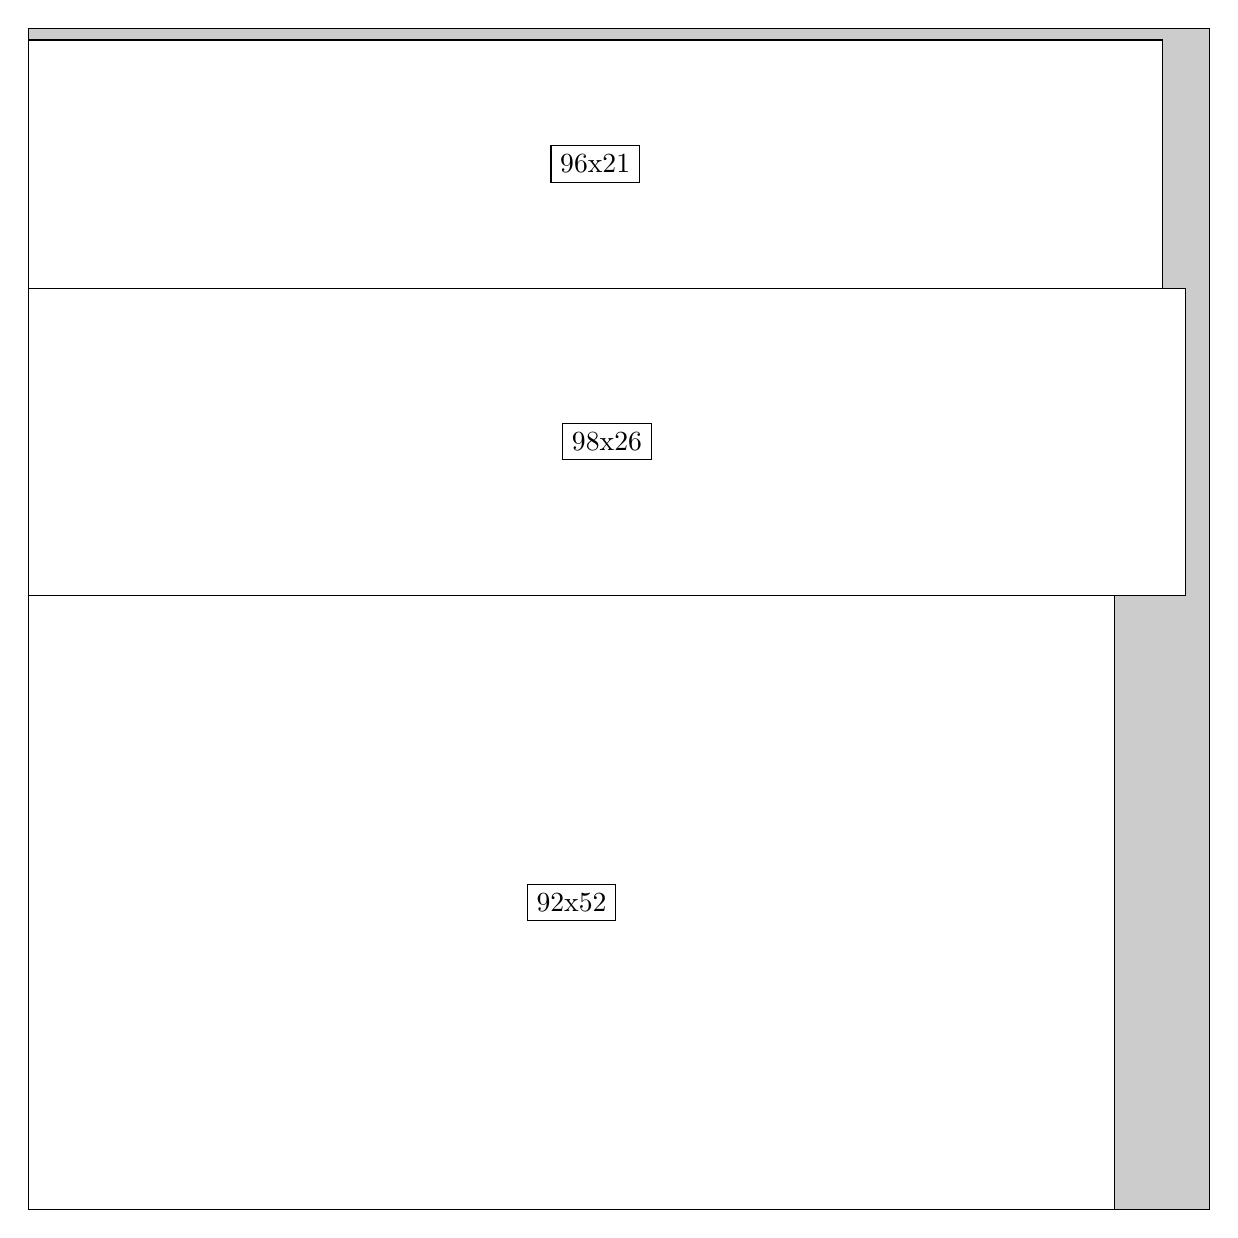
\begin{tikzpicture}[shorten >=1pt,scale=1.0,every node/.style={scale=1.0},->]
\tikzstyle{vertex}=[circle,fill=black!25,minimum size=14pt,inner sep=0pt]
\filldraw[fill=gray!40!white, draw=black] (0,0) rectangle (15.0,15.0);
\foreach \name/\x/\y/\w/\h in {92x52/0.0/0.0/13.799999999999999/7.8,98x26/0.0/7.8/14.7/3.9,96x21/0.0/11.7/14.399999999999999/3.15}
\filldraw[fill=white!40!white, draw=black] (\x,\y) rectangle node[draw] (\name) {\name} ++(\w,\h);
\end{tikzpicture}


w =92 , h =52 , x =0 , y =0 , v =4784
\par
w =98 , h =26 , x =0 , y =52 , v =2548
\par
w =96 , h =21 , x =0 , y =78 , v =2016
\par
\newpage


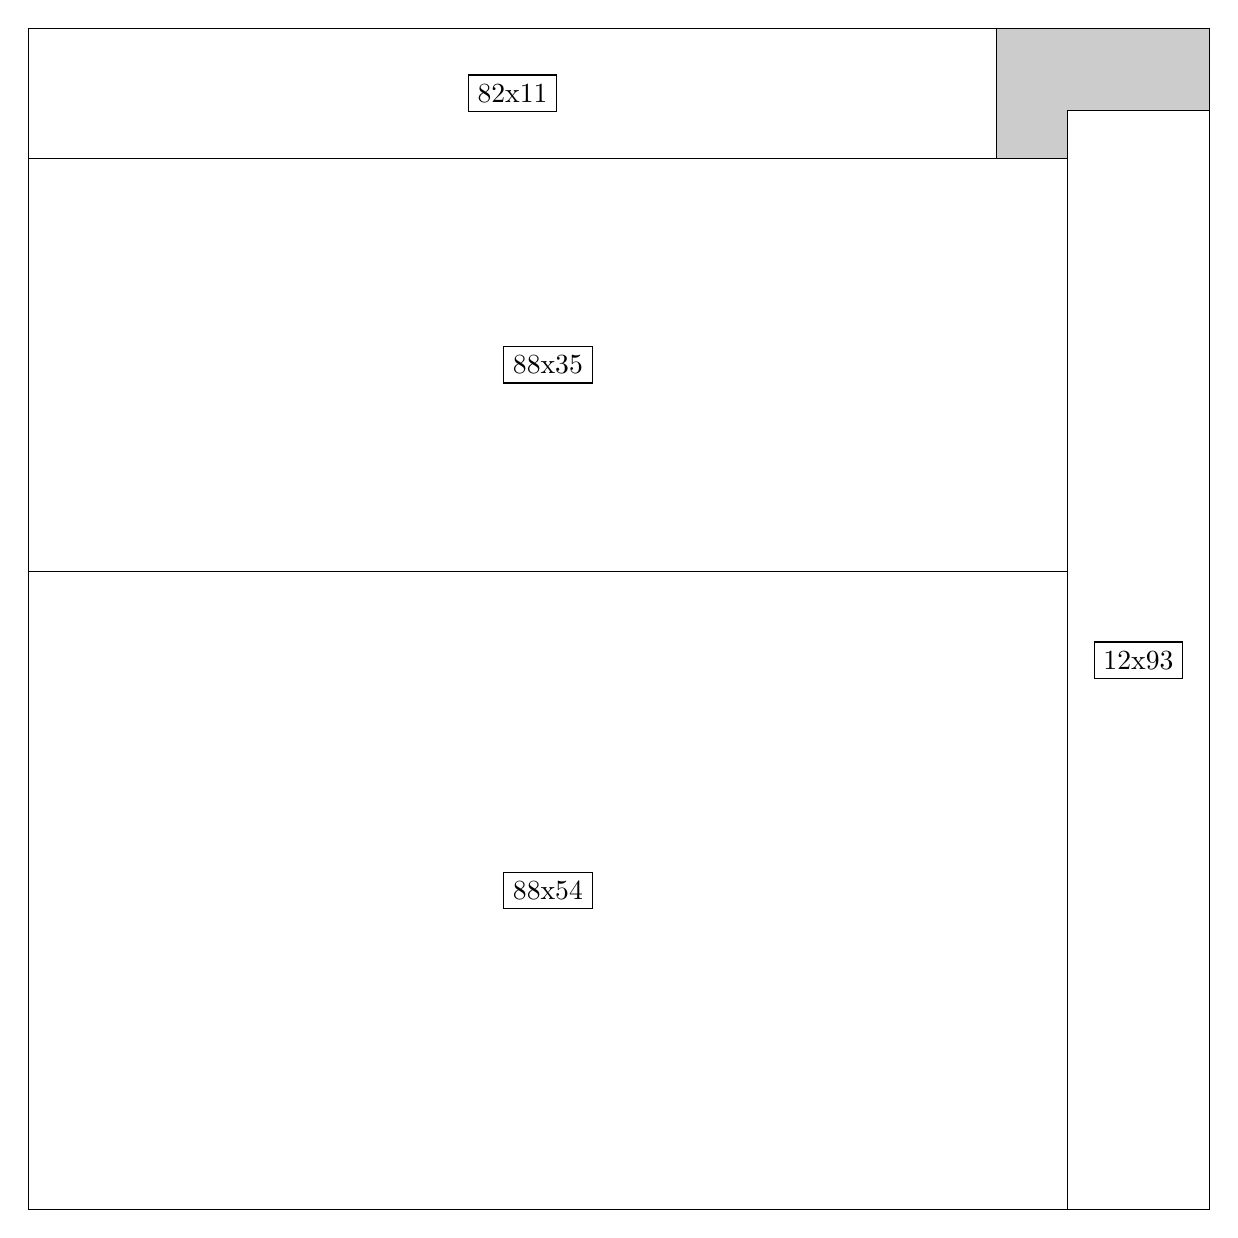
\begin{tikzpicture}[shorten >=1pt,scale=1.0,every node/.style={scale=1.0},->]
\tikzstyle{vertex}=[circle,fill=black!25,minimum size=14pt,inner sep=0pt]
\filldraw[fill=gray!40!white, draw=black] (0,0) rectangle (15.0,15.0);
\foreach \name/\x/\y/\w/\h in {88x54/0.0/0.0/13.2/8.1,82x11/0.0/13.35/12.299999999999999/1.65,88x35/0.0/8.1/13.2/5.25,12x93/13.2/0.0/1.7999999999999998/13.95}
\filldraw[fill=white!40!white, draw=black] (\x,\y) rectangle node[draw] (\name) {\name} ++(\w,\h);
\end{tikzpicture}


w =88 , h =54 , x =0 , y =0 , v =4752
\par
w =82 , h =11 , x =0 , y =89 , v =902
\par
w =88 , h =35 , x =0 , y =54 , v =3080
\par
w =12 , h =93 , x =88 , y =0 , v =1116
\par
\newpage


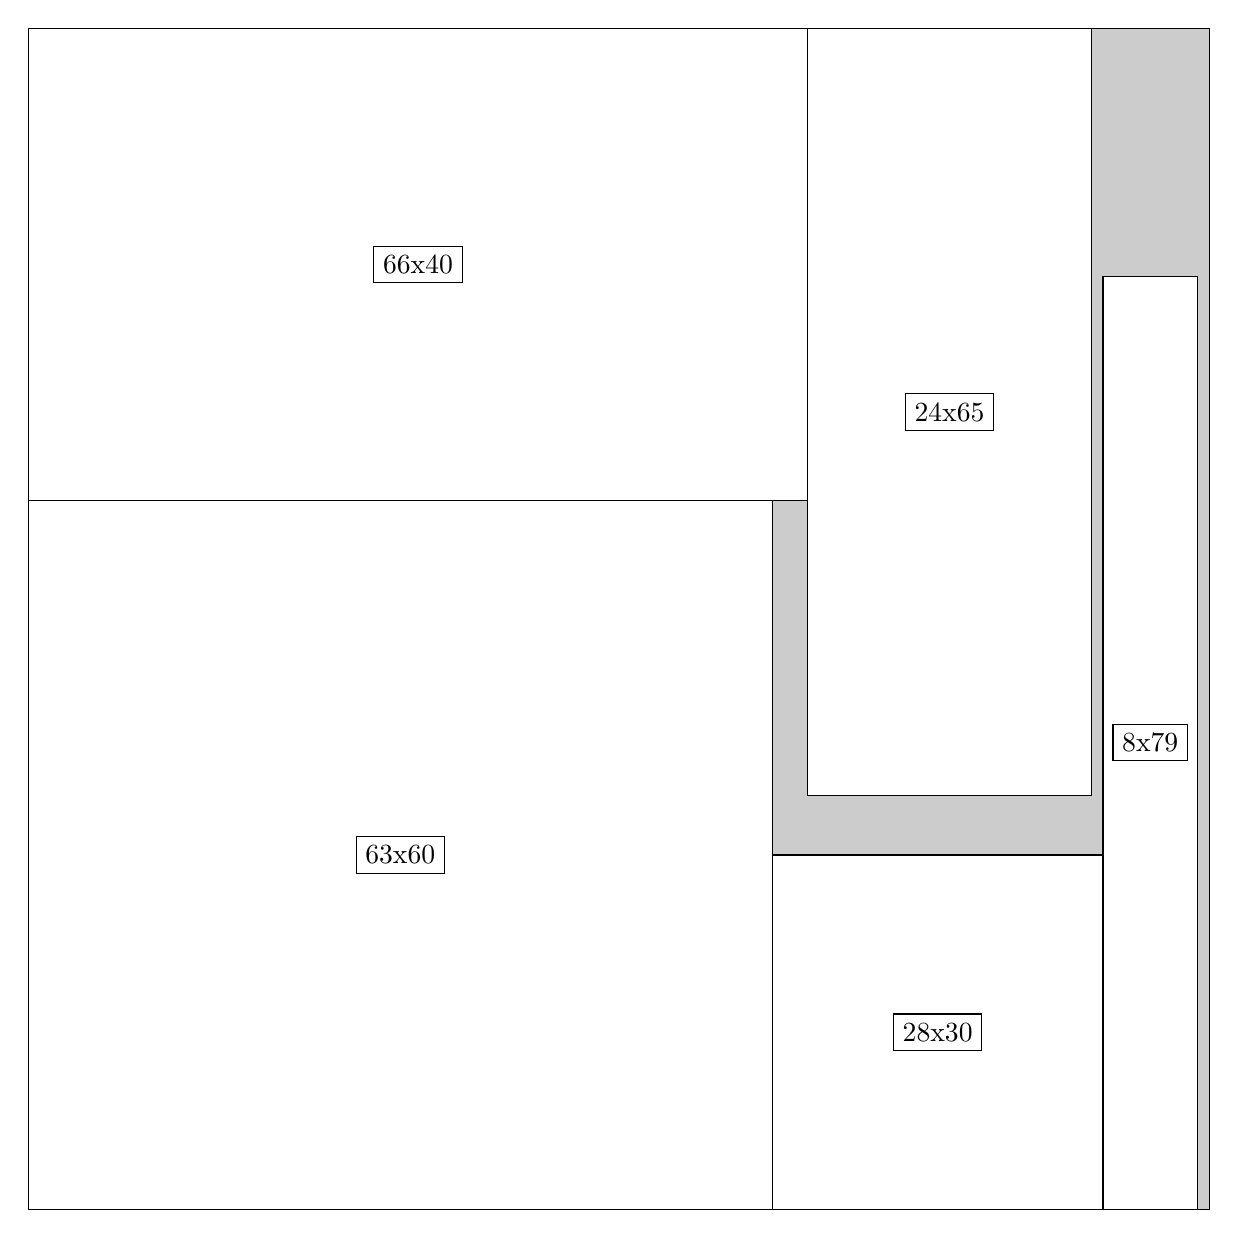
\begin{tikzpicture}[shorten >=1pt,scale=1.0,every node/.style={scale=1.0},->]
\tikzstyle{vertex}=[circle,fill=black!25,minimum size=14pt,inner sep=0pt]
\filldraw[fill=gray!40!white, draw=black] (0,0) rectangle (15.0,15.0);
\foreach \name/\x/\y/\w/\h in {63x60/0.0/0.0/9.45/9.0,66x40/0.0/9.0/9.9/6.0,24x65/9.9/5.25/3.5999999999999996/9.75,28x30/9.45/0.0/4.2/4.5,8x79/13.65/0.0/1.2/11.85}
\filldraw[fill=white!40!white, draw=black] (\x,\y) rectangle node[draw] (\name) {\name} ++(\w,\h);
\end{tikzpicture}


w =63 , h =60 , x =0 , y =0 , v =3780
\par
w =66 , h =40 , x =0 , y =60 , v =2640
\par
w =24 , h =65 , x =66 , y =35 , v =1560
\par
w =28 , h =30 , x =63 , y =0 , v =840
\par
w =8 , h =79 , x =91 , y =0 , v =632
\par
\newpage


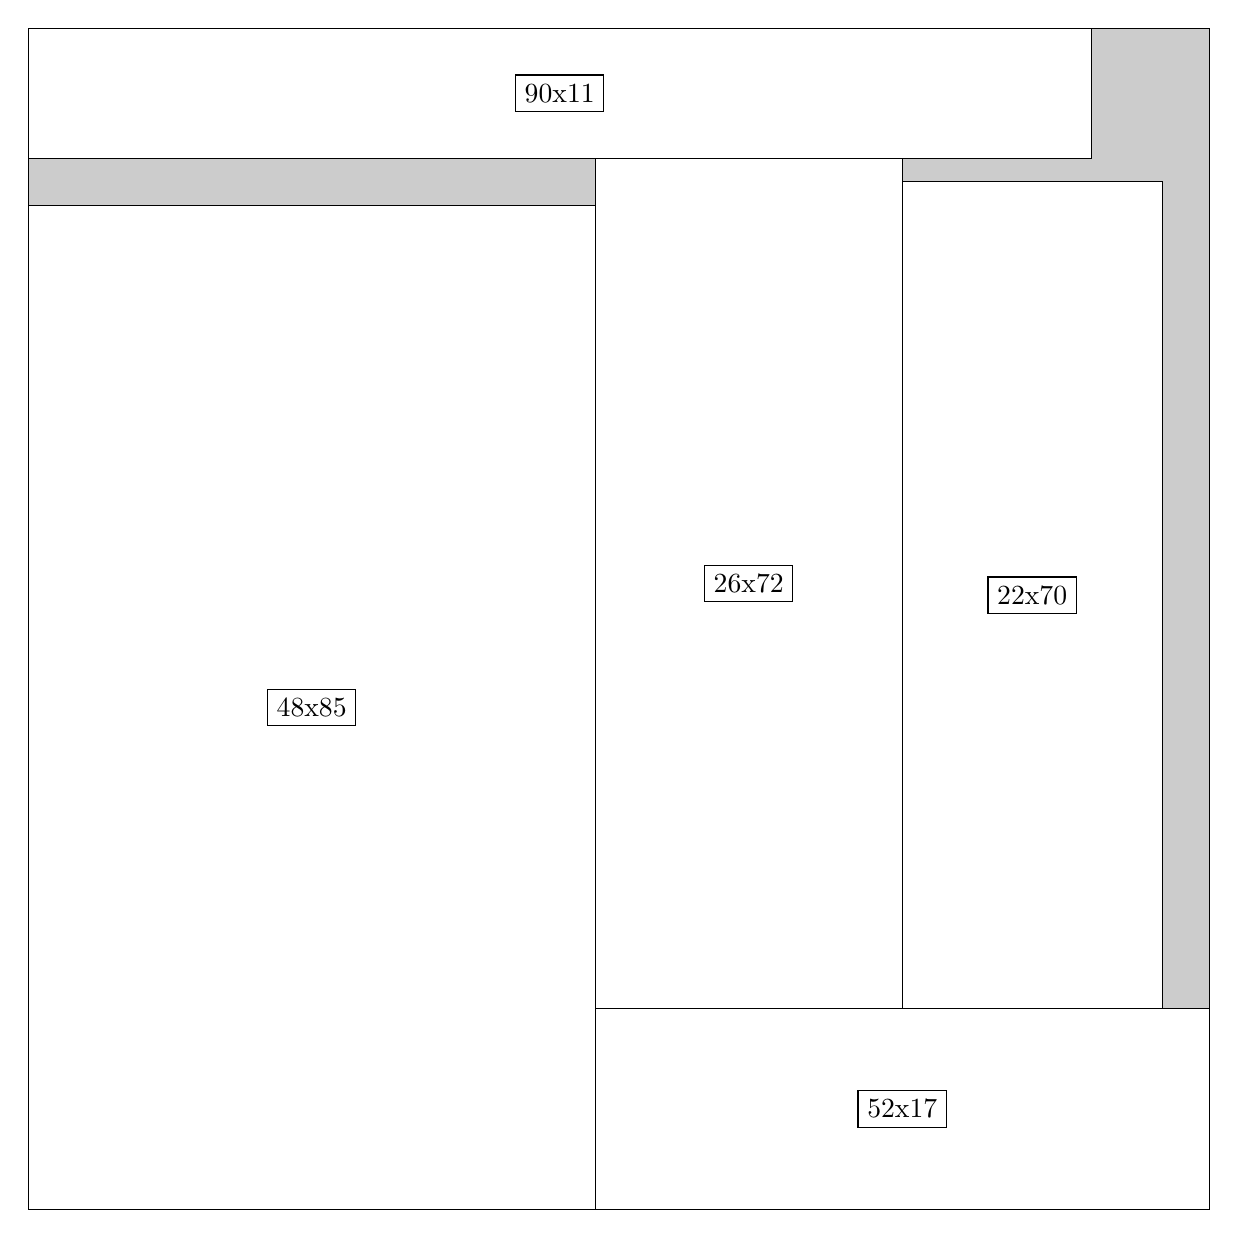
\begin{tikzpicture}[shorten >=1pt,scale=1.0,every node/.style={scale=1.0},->]
\tikzstyle{vertex}=[circle,fill=black!25,minimum size=14pt,inner sep=0pt]
\filldraw[fill=gray!40!white, draw=black] (0,0) rectangle (15.0,15.0);
\foreach \name/\x/\y/\w/\h in {48x85/0.0/0.0/7.199999999999999/12.75,26x72/7.199999999999999/2.55/3.9/10.799999999999999,22x70/11.1/2.55/3.3/10.5,90x11/0.0/13.35/13.5/1.65,52x17/7.199999999999999/0.0/7.8/2.55}
\filldraw[fill=white!40!white, draw=black] (\x,\y) rectangle node[draw] (\name) {\name} ++(\w,\h);
\end{tikzpicture}


w =48 , h =85 , x =0 , y =0 , v =4080
\par
w =26 , h =72 , x =48 , y =17 , v =1872
\par
w =22 , h =70 , x =74 , y =17 , v =1540
\par
w =90 , h =11 , x =0 , y =89 , v =990
\par
w =52 , h =17 , x =48 , y =0 , v =884
\par
\newpage


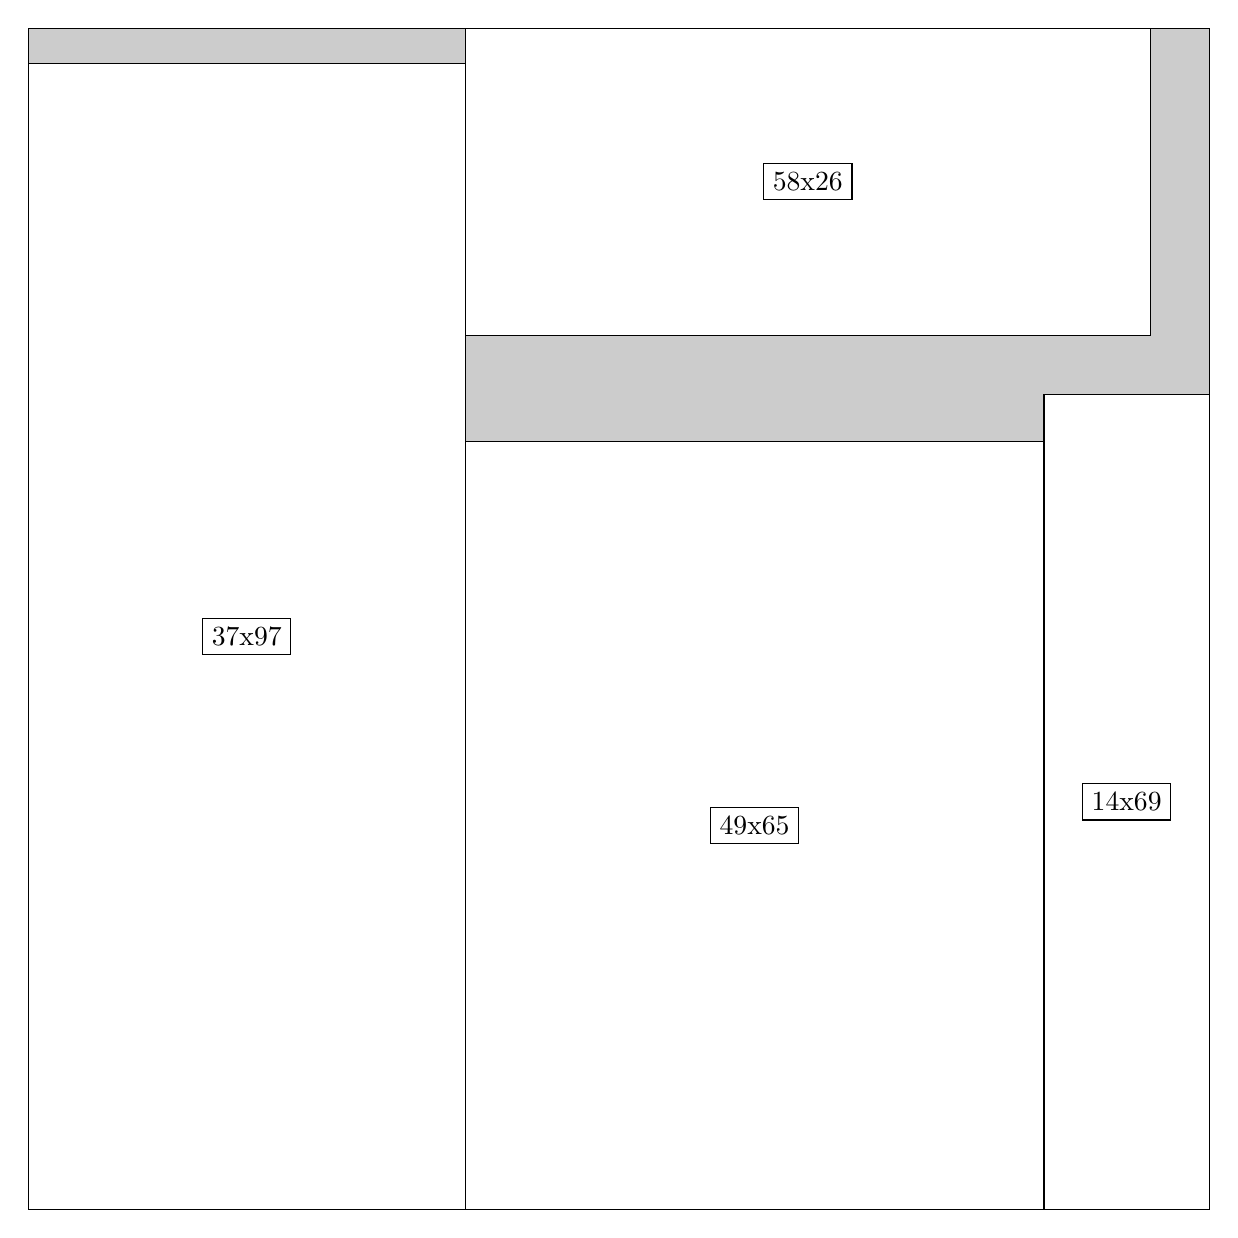
\begin{tikzpicture}[shorten >=1pt,scale=1.0,every node/.style={scale=1.0},->]
\tikzstyle{vertex}=[circle,fill=black!25,minimum size=14pt,inner sep=0pt]
\filldraw[fill=gray!40!white, draw=black] (0,0) rectangle (15.0,15.0);
\foreach \name/\x/\y/\w/\h in {37x97/0.0/0.0/5.55/14.549999999999999,49x65/5.55/0.0/7.35/9.75,58x26/5.55/11.1/8.7/3.9,14x69/12.9/0.0/2.1/10.35}
\filldraw[fill=white!40!white, draw=black] (\x,\y) rectangle node[draw] (\name) {\name} ++(\w,\h);
\end{tikzpicture}


w =37 , h =97 , x =0 , y =0 , v =3589
\par
w =49 , h =65 , x =37 , y =0 , v =3185
\par
w =58 , h =26 , x =37 , y =74 , v =1508
\par
w =14 , h =69 , x =86 , y =0 , v =966
\par
\newpage


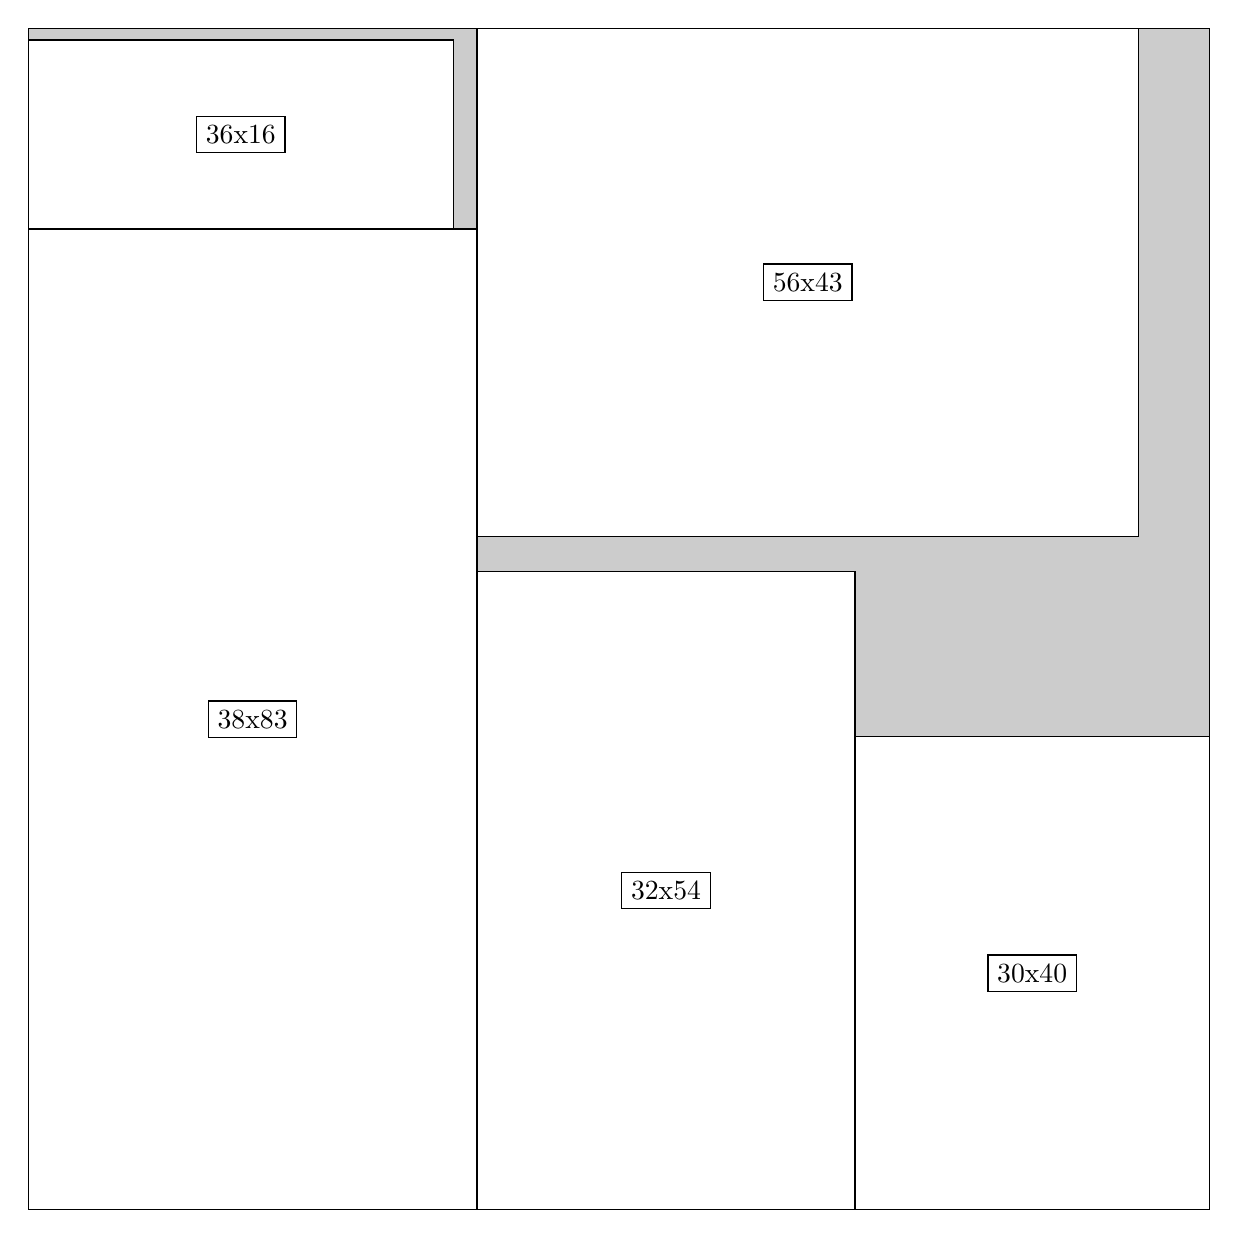
\begin{tikzpicture}[shorten >=1pt,scale=1.0,every node/.style={scale=1.0},->]
\tikzstyle{vertex}=[circle,fill=black!25,minimum size=14pt,inner sep=0pt]
\filldraw[fill=gray!40!white, draw=black] (0,0) rectangle (15.0,15.0);
\foreach \name/\x/\y/\w/\h in {38x83/0.0/0.0/5.7/12.45,56x43/5.7/8.549999999999999/8.4/6.45,32x54/5.7/0.0/4.8/8.1,30x40/10.5/0.0/4.5/6.0,36x16/0.0/12.45/5.3999999999999995/2.4}
\filldraw[fill=white!40!white, draw=black] (\x,\y) rectangle node[draw] (\name) {\name} ++(\w,\h);
\end{tikzpicture}


w =38 , h =83 , x =0 , y =0 , v =3154
\par
w =56 , h =43 , x =38 , y =57 , v =2408
\par
w =32 , h =54 , x =38 , y =0 , v =1728
\par
w =30 , h =40 , x =70 , y =0 , v =1200
\par
w =36 , h =16 , x =0 , y =83 , v =576
\par
\newpage


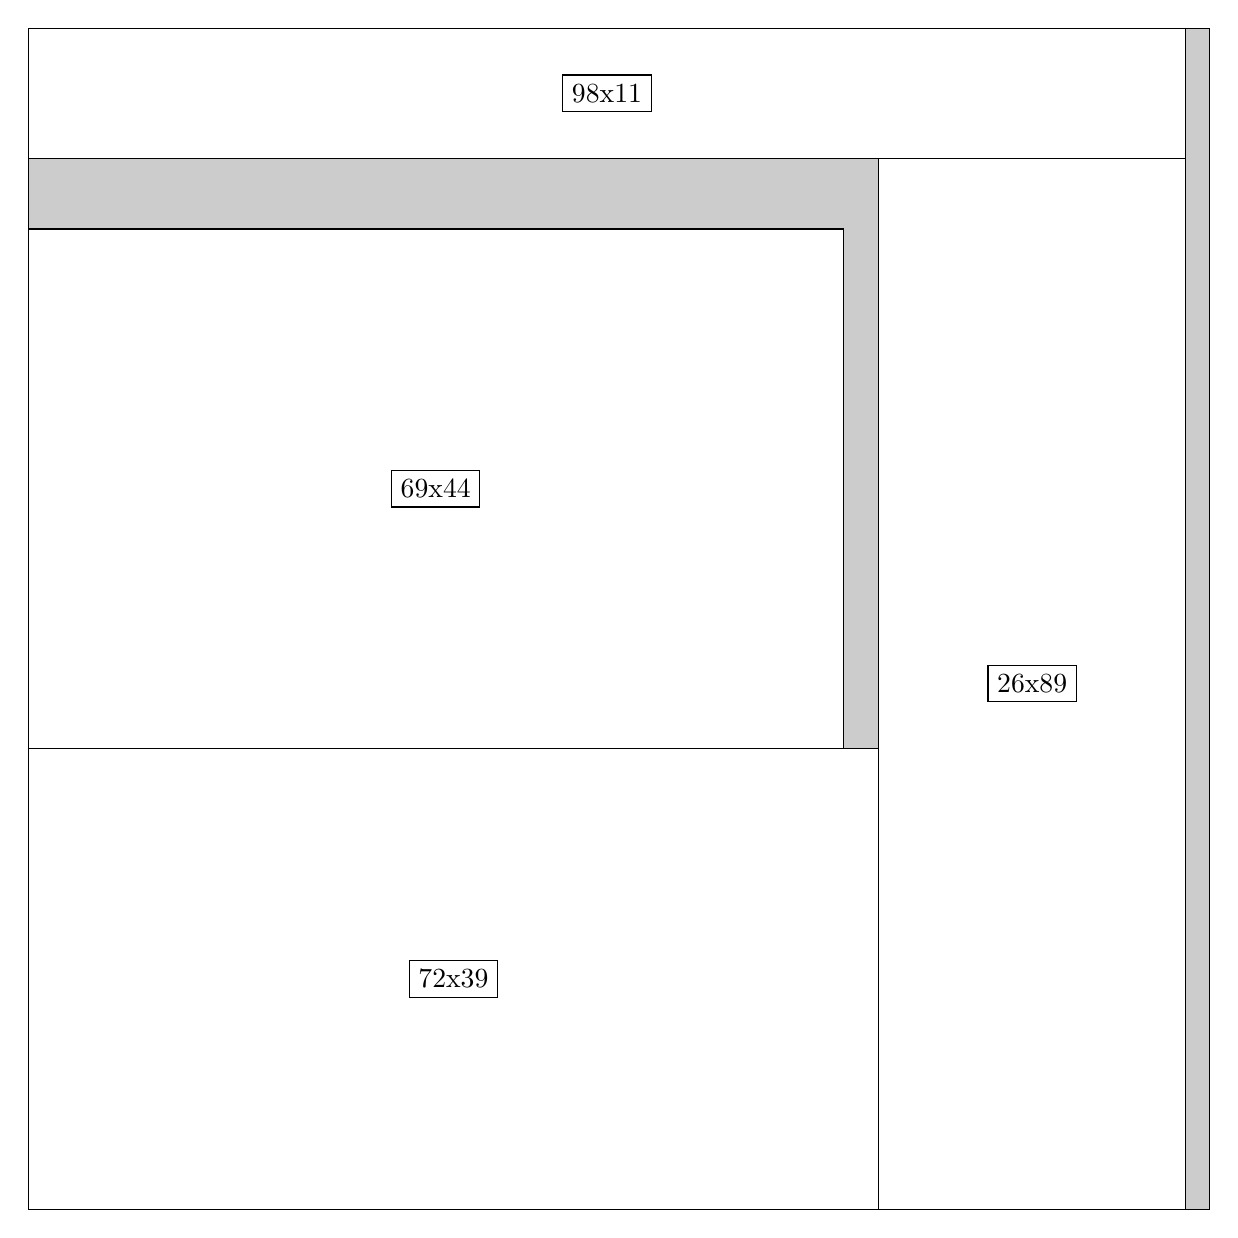
\begin{tikzpicture}[shorten >=1pt,scale=1.0,every node/.style={scale=1.0},->]
\tikzstyle{vertex}=[circle,fill=black!25,minimum size=14pt,inner sep=0pt]
\filldraw[fill=gray!40!white, draw=black] (0,0) rectangle (15.0,15.0);
\foreach \name/\x/\y/\w/\h in {72x39/0.0/0.0/10.799999999999999/5.85,69x44/0.0/5.85/10.35/6.6,26x89/10.799999999999999/0.0/3.9/13.35,98x11/0.0/13.35/14.7/1.65}
\filldraw[fill=white!40!white, draw=black] (\x,\y) rectangle node[draw] (\name) {\name} ++(\w,\h);
\end{tikzpicture}


w =72 , h =39 , x =0 , y =0 , v =2808
\par
w =69 , h =44 , x =0 , y =39 , v =3036
\par
w =26 , h =89 , x =72 , y =0 , v =2314
\par
w =98 , h =11 , x =0 , y =89 , v =1078
\par
\newpage


\end{document}